\documentclass[11pt,twoside,a4paper,titlepage]{article}
%%%%%%% Standard settings %%%%%%%
\usepackage{amsmath}
\usepackage{amssymb}
\usepackage[nottoc, numbib, notlot, notlof]{tocbibind}
\usepackage{fancyhdr}
\usepackage[utf8]{inputenc}
\usepackage{mathtools}
\usepackage{microtype}
\usepackage[svgnames]{xcolor}
\usepackage{newclude}
\usepackage{siunitx}
\usepackage{booktabs}
\usepackage{subfig}
\usepackage{wrapfig}
\usepackage[subfigure]{tocloft}
%\usepackage{todonotes}
\usepackage[disable]{todonotes}
\usepackage{lastpage}
\usepackage{lipsum,lastpage}
\usepackage{hanging}
\usepackage{tabularx}
\setlength{\headheight}{15pt}
\usepackage{filecontents}
\usepackage{longtable}
\usepackage{footnote}
\setcounter{tocdepth}{2} % Number of layers in table of content
\setcounter{secnumdepth}{5} % number of layers in sections
\usepackage[toc,page]{appendix} % appendices
\usepackage{gensymb}
\usepackage{chngcntr}
\counterwithin{figure}{section}
\counterwithin{table}{section}
\counterwithin{equation}{section}
% % Two paged margin:
% \usepackage[margin=2.5cm, inner =3cm,outer =2cm]{geometry}
% % One paged magin:
\usepackage[margin=2.5cm]{geometry}
\usepackage{paralist}
\let\itemize\compactitem
\let\enditemize\endcompactitem
\let\enumerate\compactenum
\let\endenumerate\endcompactenum
\let\description\compactdesc
\let\enddescription\endcompactdesc
\pltopsep=1pt
\plitemsep=1pt
\plparsep=1pt
%%%%%%% FIGURES %%%%%%%
\usetikzlibrary{positioning} % in the preamble
\usetikzlibrary{decorations.pathreplacing}
\usetikzlibrary{arrows,shapes}
\usepackage{tikz-timing}
\usepackage{graphics}
\usepackage{siunitx}
\usepackage{tikz}
\usetikzlibrary{shapes,arrows,chains, scopes}
\usepackage{pgfplots}
\usepackage{tabu}
\pgfplotsset{compat=1.8} % Should be supported on all machines.
\usepackage[americanvoltages, americancurrents, americanresistors, americaninductors, smartlabels]{circuitikz}
\usepackage{graphicx} % used for MATLAB figures in the format .eps
\usepackage{epstopdf} % Used for automatic convertion of .eps to pdf; Without this we cannot compile with pdfLaTeX.
\usepackage{mathtools}
\usetikzlibrary{arrows,automata} % For drawing state machines
%%%%%%% captions settings %%%%%%%
\usepackage[round]{natbib}
\bibliographystyle{plainnat}
%%%%%%% captions settings %%%%%%%
\usepackage{caption}
\captionsetup{font=footnotesize}
%%%%%%% Implimentation of C code %%%%%%%
\usepackage{listings}
\lstset{frame=tb,
tabsize=4,
language=C,
captionpos=b,
tabsize=3,
frame=false,
numbers=left,
numberstyle=\tiny,
numbersep=5pt,
breaklines=true,
showstringspaces=false,
basicstyle=\ttfamily,
% identifierstyle=\color{magenta},
keywordstyle=\color[rgb]{0,0,1},
commentstyle=\color{ForestGreen}\ttfamily,
morecomment=[l][\color{brown}]{\#},
stringstyle=\color{red}
}
%Figure text under code snippits
\renewcommand\lstlistingname{Codesnippit}
%%%%%%% Misc %%%%%%%
\usepackage{icomma}
\usepackage{pdfpages}
\usepackage[pdftex,
hyperfigures=true,
pdfauthor={Forfattere},
pdftitle={},
pdfsubject={},
pdfkeywords={},
hidelinks,
plainpages=false,
pdfpagelabels,
unicode]{hyperref}
\usepackage{textcomp,gensymb} % Adds a \degree symbol in math mode
\newenvironment{changemargin}[2]{%
\begin{list}{}{%
\setlength{\topsep}{0pt}%
\setlength{\leftmargin}{#1}%
\setlength{\rightmargin}{#2}%
\setlength{\listparindent}{\parindent}%
\setlength{\itemindent}{\parindent}%
\setlength{\parsep}{\parskip}%
}%
\item[]}{\end{list}}
%Should be used in every controller diagram - anbae12.

\tikzstyle{block} = [draw, fill=blue!20, rectangle, minimum height=2.5em, minimum width=4em]
\tikzstyle{blockgreen} = [draw, fill=green!40, rectangle, minimum height=2.5em, minimum width=4em]
\tikzstyle{blockorange} = [draw, fill=orange!60, rectangle, minimum height=2.5em, minimum width=4em]
\tikzstyle{blocknon} = [draw, rectangle, minimum height=2.5em, minimum width=4em]
\tikzstyle{freq} = [draw, fill=green!20, ellipse, minimum height=2.5em, minimum width=3.5em]
\tikzstyle{sum} = [draw, fill=blue!20, circle, node distance=1cm]
\tikzstyle{input} = [coordinate]
\tikzstyle{output} = [coordinate]
\tikzstyle{pinstyle} = [pin edge={to-,thin,black}]

\tikzstyle{zero} = [scale = 0.2, draw, circle, minimum width=1cm, thick]
\tikzstyle{pole} = [scale = 0.2, draw, cross out, minimum width = 1cm, minimum height=1cm, thick]

\begin{document}
% Disable indentation
\setlength{\parindent}{0pt}
\setlength{\parskip}{0.7\baselineskip}%
\pagenumbering{gobble}
\thispagestyle{empty}
%\begin{titlepage}


\title{Intelligent waste sorting robot}
\author{Nikolaj, Thomas, David, Xabier, Kirstine \& Simon }
\date{December 2014}

\begin{figure}[b]
\centering

\includegraphics[width=0.4\textwidth]{graphics/logo.png}
\end{figure}

\vfill
\end{titlepage}
\maketitle

\clearpage
\fancyfoot{}
\fancyfoot[CO,CE]{\thepage}
\pagenumbering{Roman}

% \section{Important information to everyone}
% I have noticed an inconsistent use of todo notes.
% To adjust for this I have made a shortcut for everyone so we can see who wrote it and it uses the same syntax.
% Just write
% \begin{verbatim}
% \name{note}          
% \end{verbatim} and the title of the section will be put in and a color will be chosen for each person.
% \nikolaj {nikolaj }
% \thomas  {thomas  }
% \david   {david   }
% \xabier  {xabier  }
% \kirstine{kirstine}
% \casper  {casper  }
% \simon   {simon   }

%%%%% Formalia should go here %%%%%%%

% \setcounter{page}{1}
\section*{Abstract}
This is where we would write our actual abstract. 
This should be clear that this is a placeholder and not the real abstract.
When we get further we should obviously write a serious one. 
\newpage
\tableofcontents
\clearpage
\listoffigures
\listoftables
\listoftodos

\pagestyle{fancy}
\fancyfoot{}of December at 12:15-13:00
\pagenumbering{arabic}
\setcounter{page}{1}
\fancyfoot[LO,RE]{\thepage}

%%%%% Content should go here %%%%%%%
\section{Collaboration}

%Introduction to Collaboration

Throughout the project the group has done several activities to improve and strengthen the collaboration. 
Good collaboration is crucial for several different reasons. 
First, it is important that we can identify each others strengths and weaknesses, so that we know which areas to have in mind when cooperating. 
Knowing each others personalities helps us collaborate. 
If everyone is comfortable expressing their opinion a better product will come out in the end. The things that have been done to improve collaboration are listed and described in this section. 


\subsection{Reflections on Use of the Group Contract}

A copy of the group contract is to be found at REFERENCE!!! \todo[inline]{Insert group contract and refer to it}

In this group, we have different experience with groupwork, some more positive than others, but we all agreed, that we wanted to take this project seriously. For this reason we found the group contract redundant. 
The main points we decided to put into the contract was that everyone had to show up on time for group meetings, or at least let the group know they were late. We also decided on an agenda for group meetings. The consequence of not following the rules are that a warning will be given, and if no improvement a second warning could kick you out of the group. 

This is a sensible group contract if everyone is serious and commited to the project, but then it is redundant anyway. It was decided in the group that this was good enough for us. 

Throughout this project we have had problems communicating and getting everyone to attend. The meetings have been weakly defined and chaotic. 
Looking back, we should have been much more specific making the group contract. It should have had more concrete consequences to be late to a meeting, or to not meet deadlines. There should also have been a guideline to figure out who should write the summeries of the group meethings, etc. 

One thing that could have helped was to have a system where if you are late, you pay a fee, or bring cake or something. This would give the small violations of the rules a small consequence. 
For the group meetings, it would have been a good idea to have a group leader and a secretary, so there was always someone who made sure to follow the agenda, and someone who wrote everything down. This could be either changing from each meeting or different people every time. A good idea would be to use the Belbin profiles to choose who should have which roles. 

Other details, like which programs the report should be written in, and which programs should be used to store it, could also have been added, to stop all later confusion. 

Looing back, we realize that a more precise groupcontract would have benefitted the group. 








\subsection{Competence Triangle}

\tikzstyle{theo} = [font=\footnotesize, rotate=60,  draw, rectangle, fill=blue!10, text=black, text width = 3.7em, minimum height =4.1em, text centered, node distance=1.7cm]
\tikzstyle{exp} =  [font=\footnotesize, rotate=-60, draw, rectangle, fill=blue!10, text=black, text width = 3.7em, minimum height =4.1em, text centered, node distance=1.7cm]
\tikzstyle{pers} = [font=\footnotesize,             draw, rectangle, fill=blue!10, text=black, text width = 3.7em, minimum height =4.1em, text centered, node distance=1.7cm]

\begin{figure}[!ht]
\centering
\begin{tikzpicture}[scale=0.7, every node/.style={scale=0.7}]
\node[draw, very thick, regular polygon,regular polygon sides = 3, minimum width= 7cm] (strengths) at (0,0) {};

\node[rotate=60, yshift=-0.5cm, xshift=-0.3cm] (theoretical) at (strengths.135) {Theoretical knowledge};
\node[rotate=-60, yshift=-0.5cm, xshift=0.3cm] (experience) at (strengths.40) {Work skills and Experiences};
\node[yshift=0.5cm] (personal) at (strengths.270) {Personal strengths};

\node[theo, above of=theoretical, yshift = -0.2cm, xshift=-3cm] (ta) {Software development (4)} ;
\node[theo, right of=ta] (tb)                                        {Electrical circuits} ;
\node[theo, right of=tb] (tc)                                        {Databases} ;
\node[theo, right of=tc] (td)                                        {Maths (3)} ;
\node[theo, above of=ta, xshift=-2.5em, yshift=-0.2cm] (te)          {Control theory} ;
\node[theo, right of=te] (tf)                                        {Energy} ;
\node[theo, right of=tf] (tg)                                        {C++ programming (2)} ;
\node[theo, right of=tg] (th)                                        {C programming (3)} ;
\node[theo, right of=th] (ti)                                        {Java programming (1)} ;
\node[theo, above of=te, xshift=-2.5em, yshift=-0.2cm] (tj)          {Physics} ;
\node[theo, right of=tj] (tk)                                        {Mechanics} ;
\node[theo, right of=tk] (tl)                                        {RE tech} ;
\node[theo, right of=tl] (tm)                                        {Lasers} ;
% \node[theo, right of=tm] (tn)                                        {Waves} ;
\node[theo, right of=tm] (to)                                        {Process management} ;
\node[theo, right of=to] (tp)                                        {Computer simulation} ;

\node[exp, above of=experience, yshift = -0.2cm,xshift=-3cm] (ea) {Teaching non experts} ;
\node[exp, right of=ea] (eb)                                      {Auto\-mation} ;
\node[exp, right of=eb] (ec)                                      {Debating} ;
\node[exp, right of=ec] (ed)                                      {Wind turbines} ;
\node[exp, above of=ea, xshift=-2.5em, yshift=-0.2cm] (ee)        {Explo\-rative} ;
\node[exp, right of=ee] (ef)                                      {Program\-ming} ;
\node[exp, right of=ef] (eg)                                      {Planning} ;
\node[exp, right of=eg] (eh)                                      {Control} ;
\node[exp, right of=eh] (ei)                                      {Carpentry} ;
\node[exp, above of=ee, yshift=-0.2cm] (ej)                       {Network handling} ;
\node[exp, right of=ej] (ek)                                      {Software solutions} ;
\node[exp, right of=ek] (el)                                      {Self improvement} ;
\node[exp, right of=el] (em)                                      {Tool handling} ;
\node[exp, right of=em] (en)                                      {Effective} ;

\node[pers, below of=personal, yshift = 0.2cm, xshift = -7.3em] (pa) {Logical} ;
\node[pers, right of=pa] (pb)                                        {Patient (3)} ;
\node[pers, right of=pb] (pc)                                        {Compre\-hensive} ;
\node[pers, right of=pc] (pd)                                        {Objective} ;
\node[pers, below of=pa, xshift=-1.85em, yshift=0.1cm] (pe)          {Humorous} ;
\node[pers, right of=pe] (pf)                                        {Team player} ;
\node[pers, right of=pf] (pg)                                        {Calm in difficult situations} ;
\node[pers, right of=pg] (ph)                                        {Analytic} ;
\node[pers, right of=ph] (pi)                                        {Realistic} ;
\node[pers, below of=pe, xshift=-4.835em, yshift=0.1cm] (pj)         {Outgoing} ;
\node[pers, right of=pj] (pk)                                        {Observant} ;
\node[pers, right of=pk] (pl)                                        {Positive (2)} ;
\node[pers, right of=pl] (pm)                                        {Structured} ;
\node[pers, right of=pm] (pn)                                        {Effective} ;
\node[pers, right of=pn] (po)                                        {Communi\-cative} ;
\node[pers, right of=po] (pp)                                        {Willing to optimize solutions} ;



\end{tikzpicture}
\caption[Competence triangle.]{Competence triangle. The qualities are divided into three categories (Theoretical knowledge, Work Skills and Experiences, and Personal Strengths), and put on the side of the triangle that matches. If more than one person in the group has the quality, the number of people having this quality, is in parenthesis.} \label{fig_triangle}
\end{figure}

In order to learn more about each group member a competence triangle was created (figure \ref{fig_triangle}). 
The competence triangle separates competences that are on a personal, theoretical and experience level. 
This is done to get a better understanding of how people view themselves and what their education involves.
Each member wrote down 2-3 things about themselves and each item and its relation to the project was discussed.

The theoretical part is covered by many technical fields, for instance math, physics and programming. 
This signals a strong area of knowledge when it comes to researching and developing solutions. 
This was used in the idea generation to what kind of product we could come up with when we combined our theoretical knowledge. The experience section covers communication by teaching and debating, but also experience from jobs. This can come in handy when you have to realize an idea. 

While everything listed in the competence triangle are things that we could provide, it shows what we cannot provide.
We do not have anyone with skills in making a business plan or idea generating.
This made us aware, very early in the process, that we would have difficulties in these areas. 
We used the provided tools, like the picture brainstorm as seen in section \ref{sec:pictures}, to generate ideas. 
The early notice about the problems we would have, gave us more time to study. 

Overall, we did not use the competence triangle a lot directly, however, it was a good tool to get us talking and we got to know each other. 
 
\subsection{Belbin}

\begin{figure} [h!]
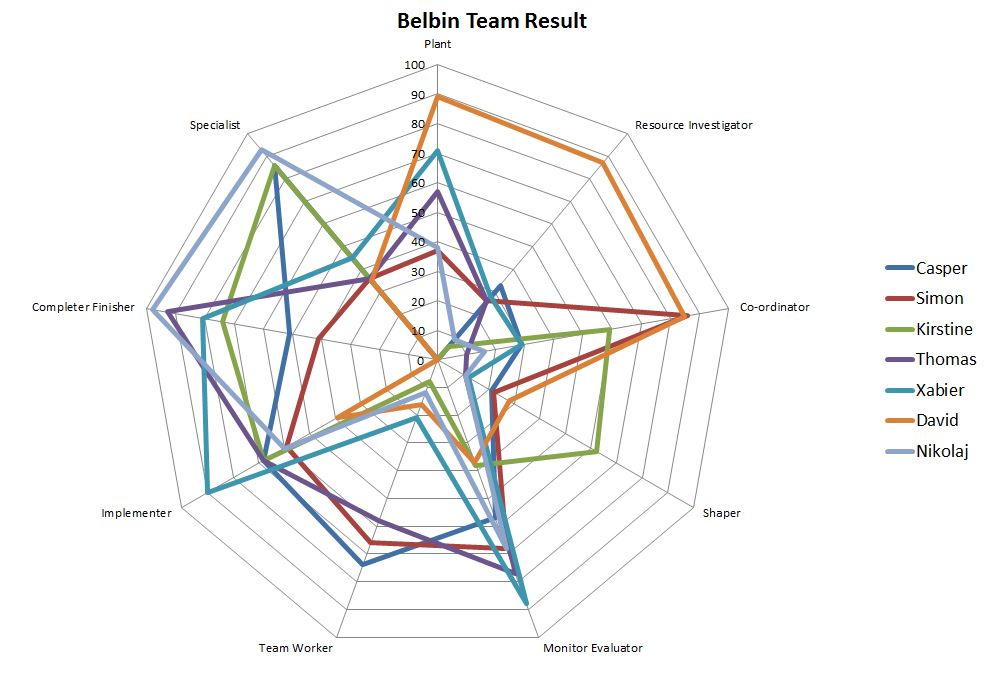
\includegraphics[width=\textwidth]{./graphics/Belbin_spiderweb}
\caption{Belbin Self-perception "Spiderweb"}
\label{belbinspider}
\end{figure}

\begin{table}[h]
\begin{tabular}{|p{0.5\textwidth}|p{0.5\textwidth}|}
\hline
\multicolumn{1}{|c|}{\textit{Contribution:}}                                                  & \multicolumn{1}{c|}{\textit{Allowable Weaknesses:}}                          \\ \hline
\multicolumn{2}{|l|}{\textbf{Top 3 roles:}}                                                                                                                                  \\ \hline
\multicolumn{2}{|c|}{\textbf{Monitor Evaluator}}                                                                                                                             \\ \hline
Sober, strategic and discerning. Sees all options and judges accurately.                      & Lacks drive and ability to inspire others. Can be overly critical to others. \\ \hline
\multicolumn{2}{|c|}{\textbf{Implementer}}                                                                                                                                   \\ \hline
Practical, reliable, efficient. Turns ideas into actions and organizes work that needs tobe done.& Somewhatinflexible. Slow to respond to new possibilities.                  \\ \hline
\multicolumn{2}{|c|}{\textbf{Completer Finisher}}                                                                                                                            \\ \hline
Painstaking, conscientious, anxious. Searches out errors. Polishes and perfects.              & Inclined to worry unduly. Reluctant to delegate.                             \\ \hline
\multicolumn{2}{|l|}{\textbf{Worst 3 Roles:}}                                                                                                                                \\ \hline
\multicolumn{2}{|c|}{\textbf{Shaper}}                                                                                                                                        \\ \hline
Challenging, dynamic, thrives on pressure. Has the drive and courage to overcome obstacles. & Prone to provocation. Offends people’s feelings.                             \\ \hline
\multicolumn{2}{|c|}{\textbf{Plant}}                                                                                                                                         \\ \hline
Creative, imaginative, free-thinking. Generates ideas and solves difficult problems.        & Ignores incidentals. Too preoccupied to communicate effectively.             \\ \hline
\multicolumn{2}{|c|}{\textbf{Resource Investigator}}                                                                                                                         \\ \hline
Outgoing, enthusiastic, communicative. Explores opportunities and develops contacts.        & Over-optimistic. Loses interest once initial enthusiasm has passed.          \\ \hline
\end{tabular}
\caption{Top/Worst 3 Belbin Self-perception for the group}
\label{belbintable}
\end{table}

This table (table \ref{belbintable}) is based on the results of the individual tests, which is also reflected by the spider web chart (figure \ref{belbinspider}). The table shows the strong and weak roles for the team profiles.

It is very clear that the group has a major potential when it comes to developing solutions to perfection, while being able to investigate the different possibilities. This could be explained by the amount of specialists in the group.

It is also very clear that the group lacks drive and a key person to set the pace of the work processes. The group has to be aware that the beginning of project is the vulnerable timespan. This is due to the missing Plants who provide creativity and innovation to the group, together with the resource investigators who makes sure the actual ideas are possible at all.
 
%Since we already encountered difficulties in the beginning of the project, it is obvious that the group is missing ideas to work with. That could also explain why we decided to go with the basic idea that was described in the project introduction papers.

%The strengths and weaknesses can all be related to the group-SWOT test.

%<Insert comparison>.
\subsection{SWOT}

Table \ref{SWOT-table} shows the SWOT-analysis of the team. 
By looking at a SWOT analysis of each person we can determine what threats can be resolved by a another group member.
If a trait is represented as both a strength and a weakness in the SWOT, they are removed. This way the SWOT will represent only the strengths and weaknesses that the group may have. This will help identify the threats the group will have to deal with.

We are very good at solving and working with problems, but at the same time we are having difficulties finding and/or creating these problems. 
This means that the team should be aware of these difficulties, especially in the beginning of the project.

We are not good at ending discussions.
To overcome this we have to remind ourselves to stop discussions when all necessary aspects have been discussed.
If we haven't resolved anything at that point we go into smaller groups so we can focus on smaller problems and to minimize group discussions.
This process breaks down issues to smaller parts so we don't end up arguing over the overall project every time we have to design a small part.

To finish small projects we delegate and spend the time to make sure that list of unfinished projects is kept to a minimum. 

\begin{table}[!ht]
\centering
\begin{tabular}{|c|c|}
\hline
\textbf{Strengths} & \textbf{Opportunities} \\ \hline
  \parbox[t]{0.45\textwidth} { %Strengths
  Our group contains people with experience with programming\\                            
  Our group is full of adaptable people with strong work ethics\\           
  We have experts on materials and sensors\\                                
  We can teach non-experts in the subjects we have an extensive knowledge\\ 
  } 
&
  \parbox[t]{0.45\textwidth} { %Oppertunities
  We can make this product without hiring external experts\\
  We will meet our deadlines\\
  We can work with different areas\\
  We will have a full knowledge of the project\\ 
  } \\ 
\hline
\textbf{Weaknesses} & \textbf{Threats} \\ \hline
  \parbox[t]{0.45\textwidth} { %Weaknesses
  We are not good at idea generation      \\
  We are not good at stopping discussions \\
  Loses focused when the goal is unclear  \\
  Other projects might distract           \\
  } 
&
  \parbox[t]{0.45\textwidth} { %Threats
  The project might get delayed\\
  We might focus on the wrong things\\
  We will have a lot of lose ends\\ 
  }\\ 
\hline
\end{tabular}
\caption{SWOT-analysis}
\label{SWOT-table}
\end{table}

%% verbose swot table.. 
% \begin{table}[!ht]
% \centering
% \begin{tabular}{|p{0.45\textwidth}|p{0.45\textwidth}|}
% \hline
% \multicolumn{1}{|c|}{\textbf {Strength}} & \multicolumn{1}{c|}{\textbf{Opportunities}} \\ \hline
% Patient(2) & Problem solving(3)\\
% Tolerant & Good presenter\\
% Open minded & Broad contacts\\
% Working with others & Interested in management\\ %I am interested in management, so I can learn it for the project
% Communicative & Solve problems on time\\
% Strong work ethics (2) & Able to structure the report\\
% Adaptable & Can finish a project. \\
% Team player & Can work from somebody's schedule\\
% Open minded & Can work late\\
% Communicating & Not afraid to delegate and face impacts\\
% On time & Mindful of others and open for com-\\
% Social & munication for instance the workload\\
% & Can work in different areas\\
% Experience (work) & Idea generation\\
% Effective & Technical skills\\
% Technically skilled & Easily can learn other subjects\\
% Clever & Team worker\\
% Logic thinking &\\
% Able to prioritize &\\
% Well organized & \\
% Decisive(2) &\\
% Ambitious &\\
% Thorough &\\
% Decisive &\\
% Dedicated to solving issues/problem &\\
% Comprehensive &\\
% Discipline on my own &\\ %Discipline when it comes to working on my own
% Creativity and innovation &\\
% \hline
% \multicolumn{1}{|c|}{\textbf {Weaknesses}} & \multicolumn{1}{c|}{\textbf{Threats}} \\ \hline
% Stubborn(2) & Not a specialist\\
% Impatient & Easily get stressed\\
% Inflexible & Impatient, if others don't understand\\ %Have a hard time when there is something others do not understand
% Being on time & Might be difficult to understand\\
% Express my ideas & Bad at solving problems myself\\
% Unwilling to recognize the value of my & Bad at remembering details\\ %Bad at remembering details, can have an impact on the overview as a whole
% work & Might ignore good suggestions when focused on other/own ideas\\
% % It is the point that there i a space between [work] and [Not starter (If goal is unclear)(2)]
% Not starter (If goal is unclear)(2) & The development phase might be slowed \\
% Loses focus easily(3) & down\\ %2nd part is from line above
% Not very innovative/creative (2) & Reduced working time \\
% Overview & I like parties and going out/I prefer fun \\
% Working fully on my own & over work\\ %2nd part is from line above
% Skeptical within my area & Focus on too many areas\\
% Not a perfectionist & We might never get started\\
% Bad at keeping track of who knows what & Bad at getting ideas to startup a project\\ %Not good at keeping track of who knows what
% Meeting deadlines & Losing focus\\
% Uncomfortable with uncertainty & Need things planned in good time\\
% & Get stalled in some point of the project\\
% & Don't finish on time\\
% \hline
% \end{tabular}
% \caption{SWOT-analysis}
% \label{SWOT-table}
% \end{table}
\subsection{Analysis Tools}
To measure participation and contribution, different analysis tools becomes viable. These tools provide an overview of each members activity during timespan of the project. Two tools have been used during the process, which are described in the sections below.

\subsubsection{Group Activity Impact Tool}
 The Group Activity Impact Tool (GAIT) is used for monitoring the relative workload of all members of a team. This will assist in evenly distributing the workload, possibly increasing the overall productivity of the team. Additionally, the tool exposes any team members that are less productive than what is expected. Every task has to be manually weighted to reflect the difficulty and workload of the task. If the difficulty or workload of a task is under- or overestimated the reflection of the workload of the members given by the tool will not be correct.
This tool has been used only sparingly throughout the course of the project. Very often it has been hard to identify individual tasks and harder still to determine the importance/weight of each task. These difficulties meant that any benefits of distributing tasks using the tool did not compensate for the extra time associated with using the tool. 
 By not using any structured method of distributing tasks, other than identifying tasks (where possible) and people volunteering for any task that they find interesting, we may have skewed the relative workload of the members. Certainly, it has meant that some people have worked almost exclusively on one area within the project.
\casper{A ref to the GAIT pic}
\begin{landscape}
	\begin{figure}[h!]
		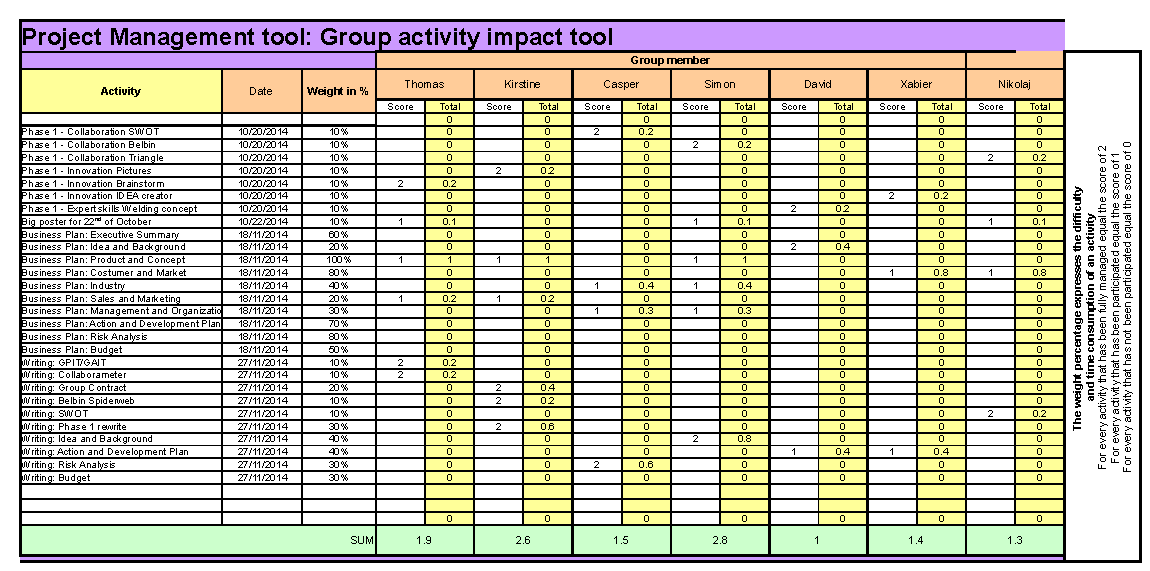
\includegraphics[scale=1.25]{./graphics/GAIT}
		\caption{The GAIT tool with tasks made by the group}
		\label{fig:GAIT}
	\end{figure}
\end{landscape}

\subsubsection{Group Participation Impact Tool}
The Group Participation Impact Tool (GPIT) is simply a tool for monitoring the meeting participation of each member. It provides a graphical representation of the participation. Using this tool will provide the team with concrete evidence of the participation of each member. This could prove useful, should a situation, where a team members contribution is in question, arise. This tool was used throughout the first month of the project but was since neglected. The results can be seen in figures \ref{fig:GPIT} and \ref{fig:GPITGraph}. Since the GPIT has only been filled out the first month, obviously, it does not give a complete image of the participation. Furthermore, according to the group contract, people agreed to working eight hours a week. These hours were not necessarily restricted to the meetings and as such this tool may not have provided us with a true representation of the actual contribution.

\todo[inline]{Update GPIT picture with names. Consider removing this altogether - It doesn't say anything meaningful.}

\begin{figure}[h!]
	\makebox[\textwidth][c]{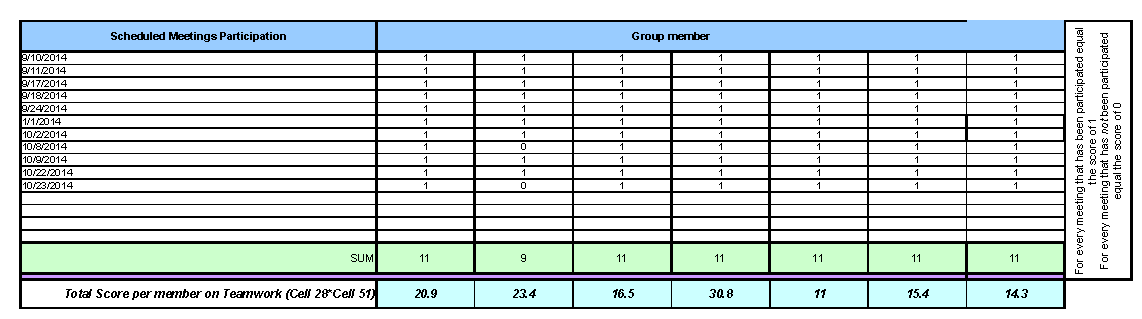
\includegraphics[scale=1]{./graphics/GPIT}}
	\caption[The GPIT tool]{The GPIT tool keeps track of attendance. If the person was there on the given date, they are given a 1.}
	\label{fig:GPIT}
\end{figure}

\begin{figure}[h!]
	\makebox[\textwidth][c]{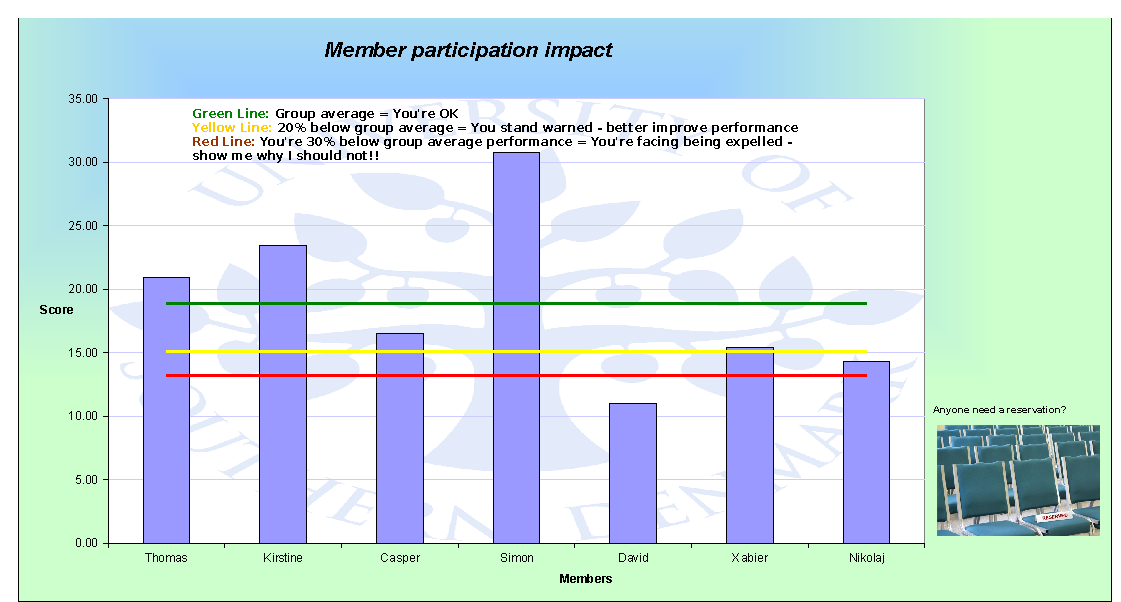
\includegraphics[scale=0.86]{./graphics/GPITGraph}}
	\caption[The contribution by each member]{The contribution to the project by each member according to the GAIT/GPIT Tools}
	\label{fig:GPITGraph}
\end{figure}
\subsection{Conclusion}
The team has had a lot of difficulties finding a problem that we wanted to work with. We have been using innovative tools including brainstorming to come up with ideas particularly around e-waste but we never got anything useful. After a meeting with the supervisors, we decided to work with an idea that was mentioned in the introduction of the project.

By looking at the results from the Belbin and SWOT-analysis it is not surprising that the team ended in the situation that we did. It is very clear that the team has a weakness when it comes to idea generation and as well a strength in problem solving. Prospectively it would be a good idea to look at the results from the team tests so we don't end up in the same situation as we already have.
%Vi har kæmpet længe med at finde det problem vi vil arbejde med, i projektet. Vi har brainstormet meget omkring affald, i sær e-affald men kom aldrig frem til noget brugbart. Efter at vores vejledere sagde at vi skulle til at komme videre, fik vi ændre projekt ide til en ide der er lagt lidt op til i projekt introduktionen.

%Ser vi på vores resultat fra Belbin og SWOT-tabellen er det ikke overraskende at vi havnede i den situation som vi gjorde. Det fremgår nemlig meget tydeligt at vi har en styrke i problemløsning men tillige en svaghed i idégenerering.Det vil fremadrettet være en god idé at se på vores styrker og svagheder fra de team tests vi har foretaget.

\clearpage
\section{Innovation and business}
\subsection{Pictures} 
\label{sec:pictures}
For an idea generation process we all sat around the same table and passed around pictures. We started with the pictures face down so we would pick them at random. When passing the pictures around, each of us said what came to mind when looking at the pictures, always keeping in mind that we were to make a creative functional robot. We made sure not to comment on each others thoughts so all thoughts were allowed. 

It was very interesting to see how different pictures generated different thoughts. There was a picture of an opera singer, and the thoughts there were: "Loud", "Hard work", "Love for your work", "Human interaction", "Service provider", "Sound recognition" and "Training algorithms". 
Another picture was of a cellphone and the thoughts there were: "Interface", "Monitoring", "Portability", "Connectivity", "Extension/Multi-functional", "Compact", "User experience", "New experience", and "Awareness/focus". 

\begin{figure}[ht]
\centering
  \begin{subfigure}[b]{0.3\textwidth}
    
\includegraphics[width=\textwidth]{./graphics/pavarotti}
    \caption{Picture of opera singer used in the idea generating process.}
    \label{fig:pavarotti}
  \end{subfigure}
  \begin{subfigure}[b]{0.3\textwidth}
    
\includegraphics[width=\textwidth]{./graphics/phone}
    \caption{Picture of cellphone used in the idea generating process.}
    \label{fig:phone}
  \end{subfigure}
\caption{Pictures used in the idea generating process}
\end{figure}





In the beginning of this process several of us found it to be somewhat a waste of time. It was difficult to see how a picture of an opera singer should help us design a robot. After the process, however, we all agreed that we had come up with some really good words, and a lot of them were words that we would like to describe our product, e.g.: "Mobility", "Safety", "Combined knowledge", "Service provider" and "Precision". Other words we would have to make sure would not end up describing our product, e.g.: "Loud", "Danger", and "Legal issues". 
\subsection{Business Model Creator (IDEA - BMC)}
\begin{figure}
%   \includegraphics[width = 0.5\textwidth]{./graphics/} %what picture did you want to include?

\end{figure}

After defining the business idea we wanted to specify problems that our idea could solve. 
To get the maximum potential from our idea, a business plan will be created. 
Creating a business plan will help in answering the question of how to generate a positive cashflow as well as generating value for customers. 
Additionally, it will help us defining our current situation and deciding which direction to take. The following sections explain the steps that were taken in developing the business model for our company.

\subsubsection{Value Proposition}
The Value proposition is a crucial part of the business model and should help us define both the services and the product that we would like create a business model for. 
Since this part could potentially assist in devoloping our project, it was chosen to start with this part.

Our expected customer base are companies in the manufacturing industry which utilize welding as part of their non-mass production chain. 
Additionally we expect to be able to sell our technology to companies which supply the industry with welding equipment. 
A company that decides to implement our technology will see a significant increase in flexibility and as such, gain an advantage in an increasingly competitive market. 
The increased flexibility will allow for futher customization of products and a reduction in both manufacturing costs and time.

It is important to us that our product is economically viable for our customers and as such we did research to determine whether there is room for a product like ours on the market.
Not surprisingly, there is a great demand for flexibility, especially amongst smaller production companies. 
We believe that our product can provide this flexibility.
However, for SME's cost is everything. By pricing our product to suit the current market price of other welding solutions, we ensure that it is seen as a viable, competitive option for SME's.

Will have to make the following comments in reference to the product configuration:
\todo[inline]{What?}

\begin{itemize}
\item We are a trusted partner in a highly integrated value chain. Our focus lies on adding value in an already established market.
\item \todo[inline]{This as alternative to next point} In order to always have the latest technology available to aid in devoloping sensory equipment for automation of welding robots, it is important that we maintain a strong relation with our partners.
\item As we focus on developing the technology necessary for the development of sensing system lines for automation of welding, a strong relation with our partners will be necessary, as we need the rest of the technology and components, in order to create the full product.
\todo[inline]{Our processes.. What does this mean? Is it significant?}
\item Our processes will be quite the same as the industrial production in general:
\begin{itemize}
\item Inbound logistics
\item Production
\item Outgoing logistics
\item Sales and marketing
\end{itemize}
\end{itemize}

\subsubsection{Finances} 
\todo[inline]{Does this mean that we have to define different products with different specifications?!}
The price of the product depends highly on the included features. 
The more or the better the features, the higher the price. Naturally, the product will be more expensive if we have to develop a new type of product with different specifications than if they buy the standard product. We will make a price list suitable to all kinds of potential customer's production.
\todo[inline]{This seems a tad short for such a huge part of a company?}
\subsubsection{Customer Configuration Table}
\todo[inline]{Short: what is this why is it important}
Finally, we have the customer configuration table as seen in table \ref{tab_conf}. 
We have a narrow area of focus, but this means that we can develop the product in response to customer needs.
\todo[inline]{Does the next part make sense when our product is distributed through... distributers? Also, don't tell people our product isn't cheap - you'll never hear apple say their products are expensive..}
As this is not a cheap product and the market is not that big, we will try to keep our customers through loyalty programs, where customers are rewarded for remaining loyal to our product. 
We believe that keeping customers happy with our products and services will assist in acquiring new customers through word of mouth. Even if our customers would rather that their competition will not gain part in the advantage that they have gotten in our product, hiding a success will not be possible for long.

\todo[inline]{Make sure this table matches the rest - potentially make a pdf from excel. urrghh..}
\begin{table}[ht]
\centering
\begin{tabular}{|m{2cm}|m{2cm}|m{2cm}|m{2cm}|m{2cm}|m{0.1cm}}%for some reason does the last cell not follow this rule so I added an invisible cell...
\rowcolor{Green}
\multicolumn{5}{l}{Customer Configuration}\\
\rowcolor{Green}
\multicolumn{2}{l}{Channel}\\
\cline{1-5}
Channel            &  Awareness        &    Evaluation    &     Purchase     &   After Sales   &\\\cline{1-5}
Internet           &  \(\mycheckmark\) & \(\mycheckmark\) & \(\mycheckmark\) & \(\mycheckmark\)&\\[1cm]\cline{1-5}                                                                       
Product brochures  &                   & \(\mycheckmark\) &                  &                 &\\[1cm]\cline{1-5}
Journals           &  \(\mycheckmark\) &                  &                  &                 &\\[1cm]\cline{1-5}
\end{tabular}
\caption{Customer configuration \label{tab_conf}}
\end{table}


\subsection{Brainstorm}
One of the main techniques applied in the ideation process was brainstorming. In order to get the best outcome from this technique it is important that any idea, no matter the absurdity, is allowed on the drawing. Others may benefit from these seemingly absurd ideas. Early on in the ideation process there was a strong consensus in the group that we find our problem in the waste recycling domain. Figure \ref{fig:wasteTypesBrainstorm} shows the first brainstorm the group made.

\begin{figure}[!ht]
	\centering
	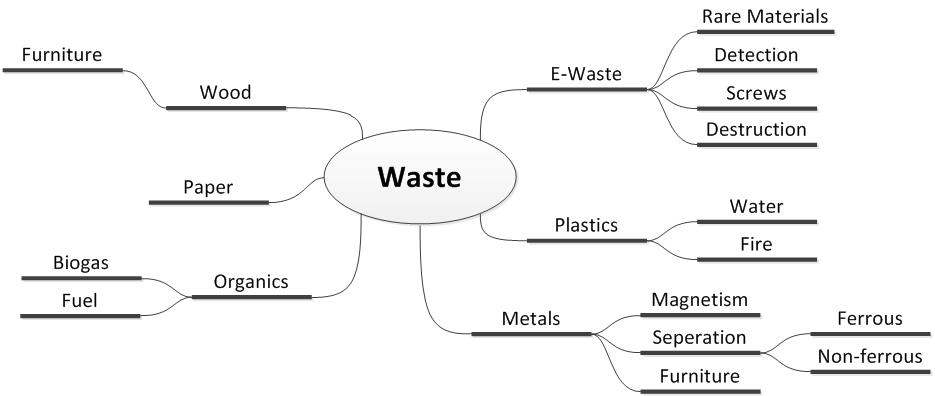
\includegraphics[scale=.5]{./graphics/wasteTypesBrainstorm.jpg}
	\caption{Brainstorm on different areas of waste recycling and possible ways of sorting}
	\label{fig:wasteTypesBrainstorm}
\end{figure}

As can be seen, the two fields of metals and E-waste received the most interest. A vote was held to decide which of the two fields we were going to continue our research on. E-waste was chosen. To further specify the problem of our project another brainstorm was started, this time on different problems within the field of E-waste. The result can be seen in figure \ref{fig:EWasteBrainstorm}.

\begin{figure}[!ht]
	\centering
	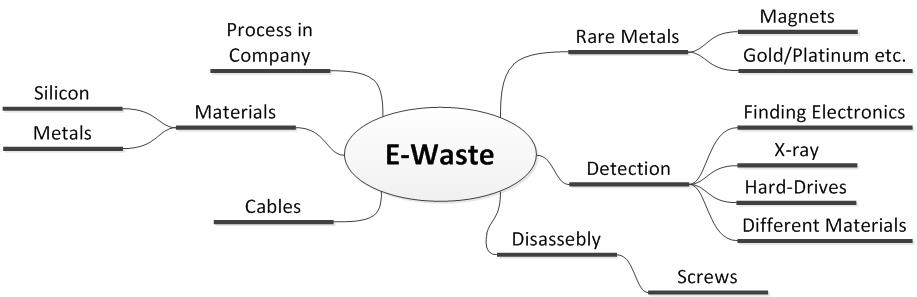
\includegraphics[scale=.5]{./graphics/EWasteBrainstorm.jpg}
	\caption{Brainstorm on problems within the field of E-Waste}
	\label{fig:EWasteBrainstorm}
\end{figure}

No real result came from the brainstorm on E-Waste, and we came to the realisation that more research was needed for us to finalize our project idea. A list of questions was devised and each member was assigned to do research on some of these questions. \\~~\\
At this point we were advised by the supervisors to either make a choice based on the research we had already done, or to go in another direction entirely. It was decided to do a brainstorm entirely focused on concepts, this can be seen in figure \ref{fig:conceptsBrainstorm}.

\begin{figure}[!ht]
	\centering
	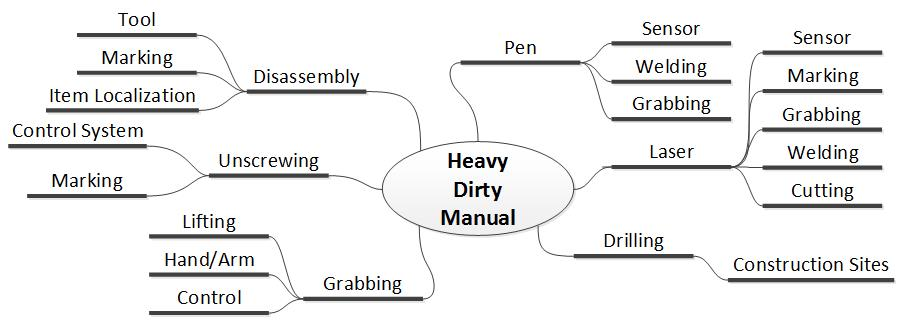
\includegraphics[scale=.5]{./graphics/conceptsBrainstorm.jpg}
	\caption{Brainstorm on possible concepts}
	\label{fig:conceptsBrainstorm}
\end{figure}

Upon finishing the brainstorm the team split into two groups, each group discussing applications for each concept. Ultimately, we decided to focus our project on the development of a flexible welding robot, using a derivation of the pen principle.

% \begin{landscape}
% 
% \begin{figure}
% \centering
% 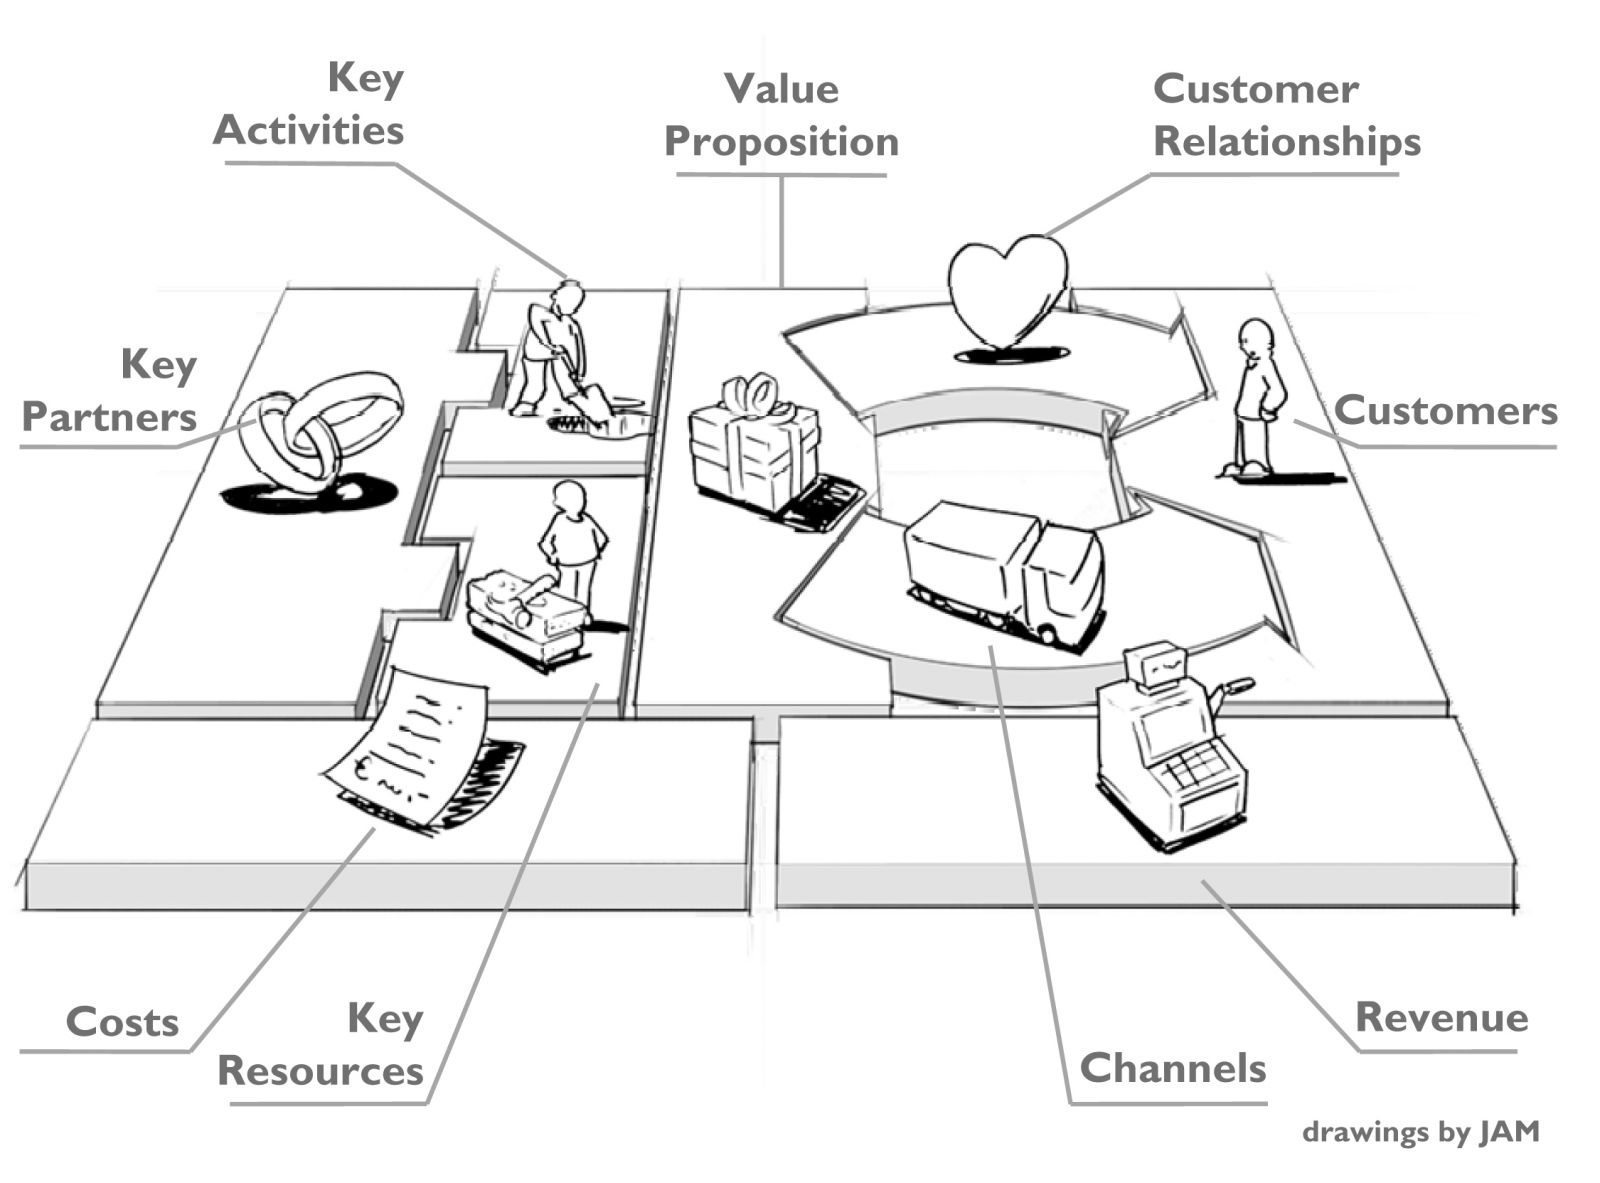
\includegraphics[width = \textwidth]{./graphics/osterwalder}
% \end{figure}
% 
% \end{landscape}



\clearpage
\section{Expert skills}
\subsection{Hardware Implementation}
All parts used in our product is existing hardware that can be purchased today.
The choice of methods and hardware, as well as some of the difficulties that are expected to arise in the development process will be explained in this section.
\subsubsection{Methods and Hardware}
There are four steps to the process performed by the welding tool proposed in this report:
\begin{itemize}
	\item \textbf{Marking:            } A worker will mark the area where the weld should be performed.
	\item \textbf{Global Localization:} When the worker has marked the area to be welded on a object the robot should identify the area. This should be able to happen at a distance of up to $1.5m$. Once identified, the robot should move the tool towards the area, stopping at an appropriate distance.
	\item \textbf{Local Localization: } With the tool closer to the area to be welded, it will detect the gap between the metal surfaces and, by following the gap, record the coordinates of the welding path.
	\item \textbf{Steady Welding:     } Once the path has been recorded, it is the responsibility of the sensor system to provide the feedback necessary to ensure that the distance to the object is kept constant throughout the welding procedure. The distance and speed along with other factors such as power use is determined by the parameters set by the worker: Metal type, thickness etc.
\end{itemize}
The process is being illustrated in figure \ref{programming_state_diagram}. Following is an explanation of the methods used in each step and the potential problems associated with them.

\begin{figure}[h]
\centering
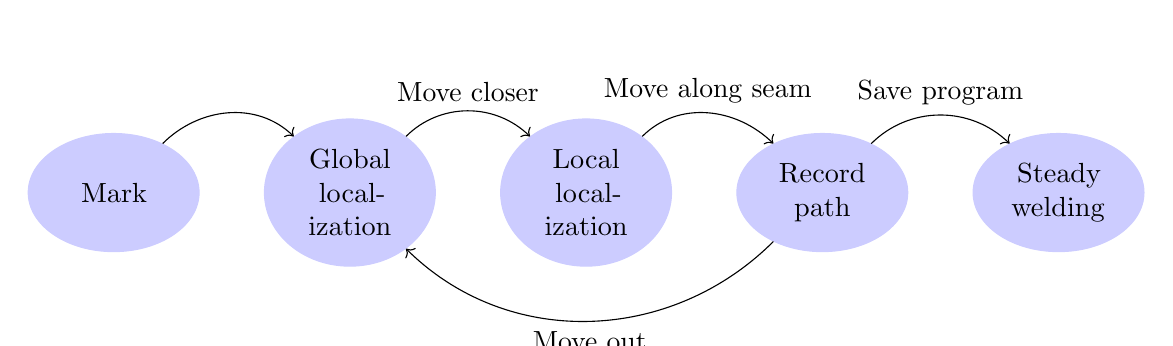
\begin{tikzpicture}[node distance=3cm]
\tikzstyle{state} = [ellipse, draw, color=blue!20, fill=blue!20, text = black, text width = 1.3cm, minimum height = 1.5cm, text centered]

\node[state, name=mark] at (0,0)            {Mark};
\node[state, name=global,  right of=mark]   {Global localization};
\node[state, name=local,   right of=global] {Local localization};
\node[state, name=program, right of=local]  {Record path};
\node[state, name=weld,    right of=program]{Steady welding};

\draw[->] (mark)     to[out=45,in=135]  node[above] {  }               (global);
\draw[->] (global)   to[out=45,in=135]  node[above] {Move closer}        (local);
\draw[->] (local)    to[out=45,in=135]  node[above] {Move along seam}  (program);
\draw[->] (program)  to[out=225,in=315] node[below] {Move out  }  (global);
\draw[->] (program)  to[out=45,in=135]  node[above] {Save program  }   (weld);
\end{tikzpicture}
\caption{Programming process with our solution}
\label{programming_state_diagram}
\end{figure}

\paragraph*{Marking}~\\
The marking will be done by colouring the area around the weld. 
Using colour will decrease the complexity of the localization process. 
However, there are a few problems associated with this approach: 
\begin{itemize}
	\item Usually you will want the area around the weld to be as clean as possible to achieve the highest quality weld.
	\item The material used for colouring should not fill out the gap between the metals.
\end{itemize}
To deal with the first issue a material that is flammable or easily deteriorated by heat could be used. 
This way the color is quickly removed when the welding process begins. 
However, the welder will need to start the weld on the coloured area, potentially lessening the quality of the first part of the weld. 
To circumvent this problem is was proposed to use a material that is deteriorated by exposure to UV light\cite{uvlight}.
This approach introduces its own problems. 
Using UV light means that anyone working in the same room as the robot should be wearing protective glasses to avoid injury. 
\nikolaj{we need reference to paint that is removed by UV light}
Additionally this also requires the tool to be fitted with a system that can do the UV light exposure, adding to the overall complexity and cost of the system.\\
The second problem requires that any material used should be sufficiently viscously and applied sparingly enough such that the gap between the metals to be welded is still detectable.

It is impossible to give all information with a marking tool alone.
There will be a touch interface on a tablet near the base of the robot that allows the user to change the settings such as metal type and welding angles. 
We aim to allow the same level of control to the workers as they have with current programming tools.
\paragraph*{Global Localization}~\\
In global localization the markings are detected.
The reasoning behind using a colouring method for marking the area to be welded is quite simply that it allows for using a camera and computer vision to do the localization. 
These are well understood, existing technologies with free options such as \texttt{OpenCV}\footnote{OpenCV: OpenCV is an open source computer vision library. www.opencv.org}. 
The tool will take a picture of the object and identify the coloured area. 
Now the tool is ready to approach the area, however it is necessary to detect the distance to the area. 
This will be done using a laser range scanner. Now, with the tool close to the object, the system is ready for the next step.
\paragraph*{Local Localization}~\\
In local localization the welding seam is detected.
At this stage the camera and laser range scanner will be used to detect the complete path that the robot must follow in order to perform a high quality weld in the desired location. 
Some problems arise at this stage:
\begin{itemize}
	\item The robot will have to be equipped with a sensory system to avoid collision with the object that is being welded upon. 
%This system will not be considered in this report and collisions are assumed to not be possible for the remainder of the report.
	\item Both while recording the path and during the welding process, it is crucial that the sensor system is maintained at the correct angle in relation to the object. 
% 	While recording the path the sensor system should be perpendicular to the object, while the angle should remain between $10-20^\circ$ when welding to obtain the highest quality weld.
\end{itemize}
In order to avoid collisions an automatic path planner will be implemented. This allows for the robot to use sensory equipment to detect whether using a specific path will result in collision with the object.
Determining the angle of the tool in relation to the object can be done using the laser range scanner and the robots positioning. This could potentially become different for every type of welding robot and thus would be problematic to develop.

When the path of a single weld has been recorded the robot will move back to find a new marked area. This leads to less motion planning as the way towards the mark was possible the robot will always find it's way back.

\paragraph*{Steady Welding}~\\
When the path has been recorded the program is uploaded and the robot will be able to follow the path.
In order to keep the welder at a constant distance to the object the laser will be used to provide feedback. 
This way the program is usable for objects where the difference is limited to assembly imperfections.
The speed of the weld as well as the distance to the object is decided on the basis of the parameters the worker has provided in the interface.
\subsection{Software Implementation}
Software is one of the essentials of the product, it is also one of the challenges for the business to exist. Since a business plan describes the fundamentals of the company and how it is going to make money, it is a critical section to describe the product, which will be done during this section. When there is a need of developing a software, the usual way would be to collect requirements from stakeholders. Currently the group is the only known stakeholder and therefore it is hard to create the usual procedure for the development. This would be a acquiring of requirements, create use cases, design a class diagram and keep it developed during the process. 

The development process is one of the key activities during the start up of the company. Therefore it is important to have focus of this specific process and making the choice of the right process. When in need of rapid development activities within the Scrum process would be attractive for the group, because it would implement the daily meeting which is used for sharing of problems and ideas for solving them. This requires an expert knowledge to become a useful process, which the group is eligible of.
\clearpage
\paragraph*{Structure of the Software System}
Figure \ref{ClassDiagram} shows the current state architecture of the software system. The system is not yet complete and will grow during the development process. The modifications are hard to predict at this very moment, but this displays the main functions of the system and what focus areas there are within the development. 
\begin{figure}[h!]
\centering
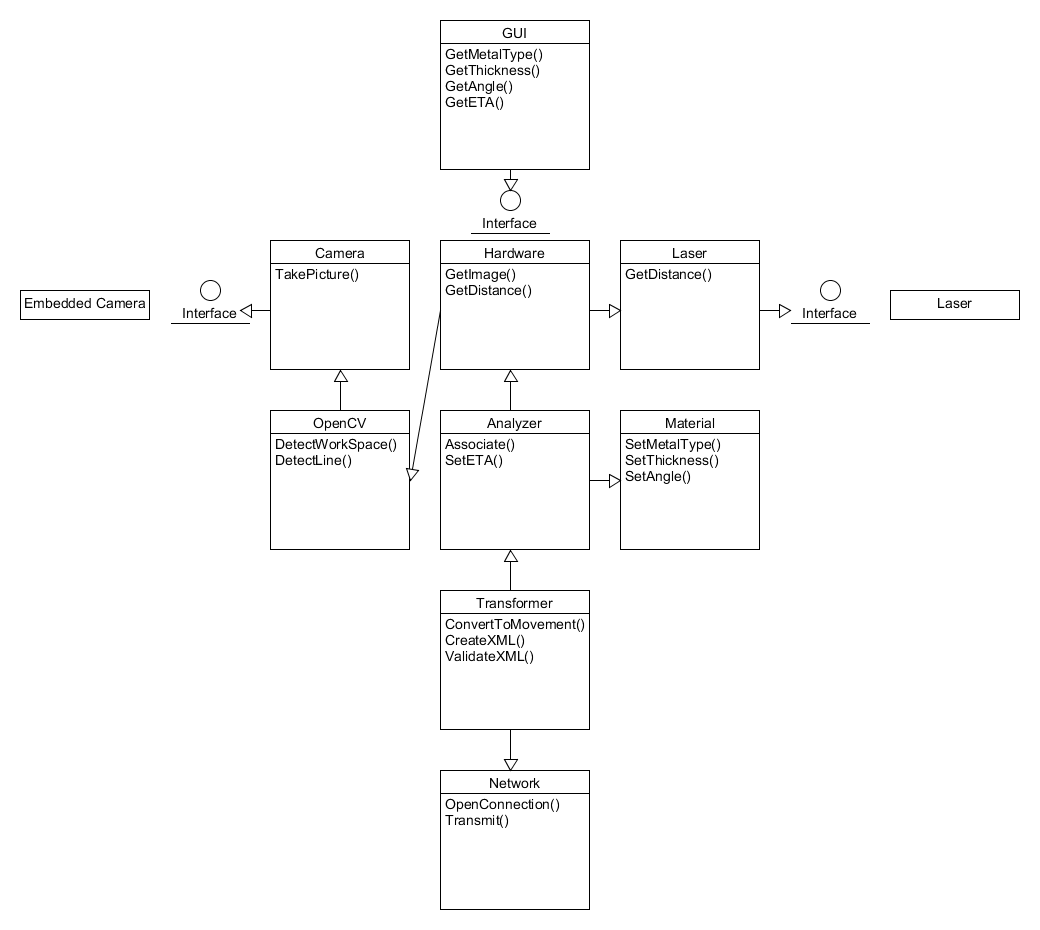
\includegraphics[width=0.7\textwidth]{graphics/ClassDiagram}
\caption{A simple class diagram for the prototype software system}
\label{ClassDiagram}
\end{figure}
\thomas{Structure/Description, same thing - revise}
\subsubsection{Description of Software Architecture}
The system is going to consist of multiple hardware parts, these parts will require interfaces for communication. This communication is going to happen not only between hardware, but also internally between different parts of the software.
In this section, these different interfaces will be described. 

\paragraph*{Hardware Interfaces}~\\
Hardware, in the form of sensors, is a major part of the product. These will require interfaces to communicate with the software system. The default software for these hardware parts does not necessarily output comparable data. The usual way to approach this issue is to implement adapter patterns, which includes a facade pattern. Below is a list of the hardware interfaces used in the system:

\begin{itemize}

\item Adapter pattern for the Laser Scanner output software
\item Network Interface between Add-On and a potential robot

\end{itemize}

Both the camera and laser scanner will come from different manufacturers, therefore there is no guarantee for compatibility of the manufacturers software. This is where an adapter pattern becomes useful within the system.

The network interface would have to fit specific standards within robotic interfaces. It is very dependant on the future partners and their choice of robotic interfaces.
  
\paragraph*{Software Interfaces}~\\
Software interfaces are often used when it comes to facade parts of a system. This helps making the objects unknown to other objects in the system. The purpose is to make a system with low coupling and high cohesion. Interfaces are also common to use when you have several objects or classes which need the same method, so to lower the amount of 'copy + paste' code, you should implement interfaces instead. It is hard to identify methods that should be reinvented within the current prototype class diagram, which is why this section will not cover them. That is why the class diagrams will be updated during the development process of the software. Here is a list of the different software interfaces used in the system:

\begin{itemize}

\item Facade pattern for the embedded camera
\item Facade pattern between user interface and logic layer

\end{itemize}

\paragraph*{User Interfaces}~\\
User interfaces require fundamental design to become useful for the end users. The design process often requires a huge amount of communication with the customers and stakeholders. User friendliness is the keyword within the design process. 

The Add-On will come with a tablet which provides the user interface. Different functionalities are provided by this interface: 

\begin{itemize}

\item Selection of material to weld 
\item Define thickness of the object
\item Welding angle of the robot
\item Overview of different data, like ETA of the current welding, range of the laser scanner

\end{itemize}

This enables the end user to modify the welding process in a few steps. Importance of user friendliness is immense, since the time spent on modifying the process has to be compared to the time the user could spend somewhere else.

\subsubsection{Specific requirements}
Requirements are fundamental to specify the tasks to solve when creating a software system. Requirements can be divided into categories, which is done below:

\textbf{Functional Requirements:}
\begin{itemize}

\item The system should be able to communicate with the specified hardware
\item The system should be able to communicate with any welding robot of potential future partners
\item The system should be able to take pictures with an embedded camera 
\item The system should be able to detect a line within the workspace of each picture provided by the embedded camera, by using OpenCV
\item The system should be able to create three dimensional coordinates based on inputs from a range scanner and a camera
\item The system should be able to convert movement-coordinates for a specific robot

\end{itemize}

\textbf{Non-functional Requirements:}

\begin{itemize}

\item The system should be able to create a path for the robot within one tenth of the time it takes to pickup the coordinates.
\item The precision of the laser should be $\pm$0.05 cm

\end{itemize}

\paragraph*{Functions}

The system can be divided into three major functions, which handles the process of detecting the place to weld, associate x,y an z coordinates and convert them into the movement program of a robot.

These actions can be divided into the following functions:

\begin{itemize}

\item \textbf{DetectLine:} Using functionality from the OpenCV library, this function is to detect the workspace area, by detecting the color marked by a worker, then detecting the line within.
\item \textbf{Associate:}This class has the task of gathering the two different data (camera coordinations and laser depth coordinations).
\item \textbf{ConvertToMovement:} The final coordinates generated from the Associate class is being converted to an input which a robot can use. 

\end{itemize}
\thomas{The list below seems like it could use an explanation for its existance? Also, do they need a paragraph each?}
\paragraph*{Dependencies}~\\
Using libraries can create dependencies within the system, mainly when a used library is dependant on other libraries. In this project, the OpenCV library will be in focus when extracting data of the line that the robot has to weld.   
\paragraph*{Database}~\\
A database to log every entry is favourable for the end customer, but it is not a part of the add-on and therefore not a part of the development process.
\paragraph*{System attributes}~\\
System attributes describes the qualities of a system in short terms. Primary qualities of the system is going to be:

\begin{itemize}

\item Reliability
\item Precision
\item Maintainability
\item Adaptability
. 
\end{itemize}
These are the attributes needed for a system to be able to adapt to any robot welding system, while maintaining its reliability and precision.
\subsubsection{Design decisions}
Basically the system is set to follow the 3 layer structure. But as the system evolves it can be hard to predict whether this is going to change or not. \thomas{surely this wont change if that's the structure we decide to use.}

A factor which is common in the industry, is the request for real time actions within a network. This is not direct request, since a worker handles the robot and leaves it for its time to work. This mean that no special BUS networks are needed within the system and that a TCP protocol Ethernet network is a viable option. \thomas{I don't quite understand the implications of this? real time? Ethernet? what?}

\subsubsection{Life cycle}

When the product has been developed and released it is far from complete, this is the reason for maintenance and repeating the working process of optimization and development. If the product is not updated, competitors and new ideas on the market will quickly surpass our product. Therefore it is important to repeat the actions described in the life cycle below:
\clearpage

\begin{figure}[ht]
\centering

\includegraphics[width=0.5\textwidth]{graphics/Software_Development_Life_Cycle}
\caption{The life cycle describes the process of establishing and maintaining a system}
\label{SDLC}
\end{figure}
\thomas{pretty graph, but needs a better explanation to be useful}
This process is not very detailed, because it is up to the developers and manage to choose a specific development process or a combination of them.


\clearpage
\section{Business plan}
\begin{landscape}
\begin{figure}
\centering
  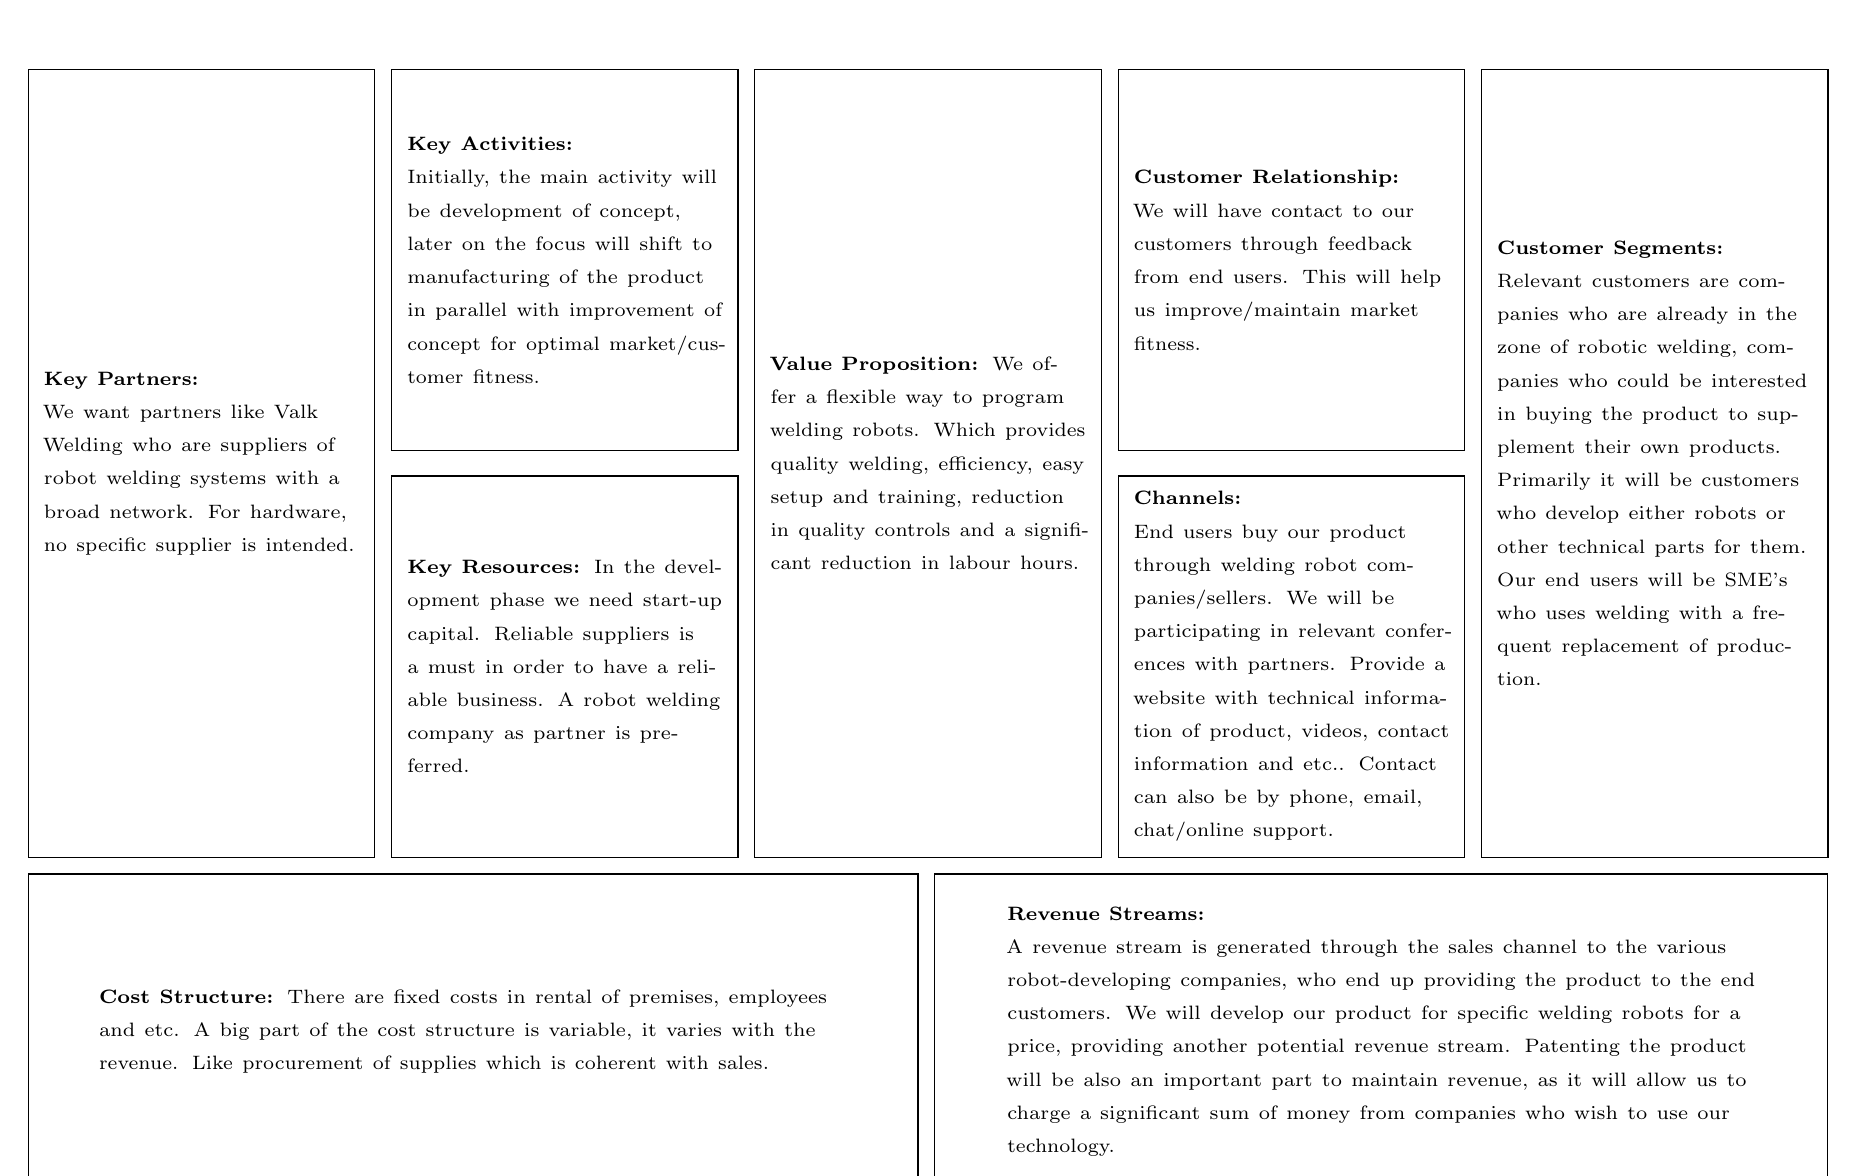
\begin{tikzpicture}[node distance=2mm,scale=1, every node/.style={scale=1}]
  \begin{scope}[start chain]
    \node[minimum height=10cm,   minimum width=4.4cm,  on chain, text width=4cm, draw, name=KP]  (0,0)                  
    {\scriptsize \textbf{Key Partners:}\\ 
We want partners like Valk Welding who are suppliers of robot welding systems with a broad network. For hardware, no specific supplier is intended.
    }; 
      \begin{scope}[start branch]
	\node[minimum height=4cm,   minimum width=11.3cm,    on chain=going below, text width=9.5cm, draw, name=CoS,xshift=3.45cm] 
	{\scriptsize\textbf{Cost Structure:}
There are fixed costs in rental of premises, employees and etc. A big part of the cost structure is variable, it varies with the revenue. Like procurement of supplies which is coherent with sales. 
	}; 
	\node[minimum height=4cm,   minimum width=11.34cm,    on chain=going right, text width=9.5cm, draw, name=RS]  
	{\scriptsize\textbf{Revenue Streams:}\\
A revenue stream is generated through the sales channel to the various robot-developing companies, who end up providing the product to the end customers.
We will develop our product for specific welding robots for a price, providing another potential revenue stream. 
Patenting the product will be also an important part to maintain revenue, as it will allow us to charge a significant sum of money from companies who wish to use our technology.
	}; 
      \end{scope}
      
      
      \begin{scope}[start branch]
	\node[minimum height=4.84cm, minimum width=4.4cm,  on chain=going right, text width=4cm, draw, name=KA,yshift=2.58cm]     
	{\scriptsize\textbf{Key Activities:}\\
Initially, the main activity will be development of concept, later on the focus will shift to manufacturing of the product in parallel with improvement of concept for optimal market/customer fitness.
	};
      \end{scope}
      \node[minimum height=4.84cm, minimum width=4.4cm,  on chain=going right, text width=4cm, draw, name=KR,yshift=-2.58cm]              
      {\scriptsize\textbf{Key Resources:}
In the development phase we need start-up capital. Reliable suppliers is a must in order to have a reliable business. A robot welding company as partner is preferred. 
      }; 
      \node[minimum height=10cm,   minimum width=4.4cm,  on chain=going right, text width=4cm, draw, name=VP,yshift=2.58cm]                
      {\scriptsize\textbf{Value Proposition:}
We offer a flexible way to program welding robots. Which provides quality welding, efficiency, easy setup and training, reduction in quality controls and a significant reduction in labour hours.
      };
	\begin{scope}[start branch]
	  \node[minimum height=4.84cm, minimum width=4.4cm,  on chain=going right, text width=4cm, draw, name=CR,yshift=2.58cm]              
	  {\scriptsize\textbf{Customer Relationship:}
We will have contact to our customers through feedback from end users. This will help us improve/maintain market fitness.
	  }; 
	\end{scope}
      \node[minimum height=4.84cm, minimum width=4.4cm,  on chain=going right, text width=4cm, draw, name=Ch ,yshift=-2.58cm]              
      {\scriptsize\textbf{Channels:}\\
End users buy our product through welding robot companies/sellers. We will be participating in relevant conferences with partners. Provide a website with technical information of product, videos, contact information and etc.. Contact can also be by phone, email, chat/online support.	
      };
      \node[minimum height=10cm,   minimum width=4.4cm,  on chain=going right, text width=4cm, draw, name=CuS,yshift=2.58cm]               
      {\scriptsize\textbf{Customer Segments:}\\
Relevant customers are companies who are already in the zone of robotic welding, companies who could be interested in buying the product to supplement their own products. Primarily it will be customers who develop either robots or other technical parts for them.  
Our end users will be SME's who uses welding with a frequent replacement of production.
      };
    \end{scope}
    

  \end{tikzpicture}
  \caption{Osterwalder Business Model}
  \label{ost_business_model}
\end{figure}
\end{landscape}

% \subsubsection{Customer segment}
% Relevant customers are companies who are already in the zone of robotic welding, companies who could be interested in buying the product to supplement their own products. Primarily it will be customers who develop either robots or other technical parts for them.  
% Our end users will be SME's who uses welding with a frequent replacement of production.
% \subsubsection{Value proposition}
% We offer a flexible way to program welding robots. Which provides quality welding, efficiency, easy setup and training, reduction in quality controls and gives a significant reduction in labour hours.
% \subsubsection{Channels}
% End users buy our product through welding robot companies/sellers. We will be participating in relevant conferences with partners. Provide a website with technical information of product, videos, contact information and etc.. Contact can also be by phone, email, chat/online support.	
% \subsubsection{Customer relationships}
% We will have contact to our customers through feedback from end users. This will help us improve/maintain market fitness.
% \subsubsection{Revenue}
% A revenue stream is generated through the sales channel to the various robot-developing companies, who end up providing the product to the end customers.
% We will develop our product for specific welding robots for a price, providing another potential revenue stream. 
% Patenting the product will be also an important part to maintain revenue, as it will allow us to charge a significant sum of money from companies who wish to use our technology.
% \subsubsection{Key resources}
% In the development phase we need start-up capital. Reliable suppliers is a must to have a reliable business. A robot welding company as partner is preferred. 
% \subsubsection{Key activities}
% Main activity in the beginning will be development of concept, later on it will be production of concept in parallel with improvement of concept for optimal market/customer fitness.
% \subsubsection{Key partners}
% We want partners like Valk Welding who is a robot welding company with a broad network. For supplies, no specific supplier is intended.
% \subsubsection{Costs}
% Where are fixed costs in rental of premises, employees and etc. A big part of the cost structure is variable, its varies with the revenue. Like purchasing of supplies which is coherent with sales. 
\subsection{Business Model}
The business model (based on the Osterwalder business model) is providing a short overview of the business plan. It will help to the company to create, deliver and capture value in economic and other contexts. It is also useful to represent core aspects of a business, such us, purpose, target customers, strategies, etc.  The model is divided into 9 categories: 
\begin{table}[h!]
\begin{tabular}{c c}
\begin{minipage}{8cm}
\begin{enumerate}
\item Key Partners
\item Key Resources
\item Key Activities
\item Value Proposition
\item Channels
\end{enumerate}
\end{minipage}
&
\begin{minipage}{8cm}
\begin{enumerate}[]
\item [6.] Customer Segments
\item [7.] Customer Relationships
\item [8.] Cost Structure
\item [9.] Revenue Stream
\end{enumerate}
\end{minipage}
\\
\end{tabular}
\end{table}

\subsection{Idea and Background}
This section briefly covers a description of the problem that we are trying to solve, how we are going to solve it.

It will also contain a short presentation of members of the team and an explanation as to why we are the perfect fit for this start up company.

\subsubsection{Problem}
The problem that we seek to solve involves flexibility within the area of industrial manufacturing. Usually a recipe is made and stored for each individual task.
Making these recipes, or reprogramming the robots is necessary whenever a new task arises and within parts of the manufacturing business this is a common occurance. 
Adaptability and precision are major keywords when it comes to welding tasks for industrial robots. Both are adjectives that do not describe current methods well.

\subsubsection{Solution}
We provide a solution to the problem mentioned above, which does not require programming. The product itself is an add-on for welding robots, that allows the robot to detect welding seams with minimal user interaction. The add-on will provide coordinates, used to create a welding-path for the robot. 

The product consists of a micro computer, which is used to make calculations based on input from a camera and a laser range scanner. 

\subsubsection{The Team}
We are a dedicated team of engineering students. We believe that we have the drive and expertise necessary to realise this project. This project is an extension of our individual interests and as such it is only natural that we extend this to our proffesional careers. Below is a presentation of all of the members of the team.

\begin{table}[h]
\centering
\begin{tabular}{|c|c|c|c|}
\hline

\includegraphics[width=0.2\textwidth]{graphics/cgopic} & %casper

\includegraphics[width=0.2\textwidth]{graphics/AnonProfile} & %david

\includegraphics[width=0.2\textwidth]{graphics/Kirstine} & %kirstine

\includegraphics[width=0.2\textwidth]{graphics/Nikolaj_profile} \\ \hline %nikolaj
\parbox[t] {0.2\textwidth}{
\textbf{Casper:} \\
28 years old, originally from Gelsted, Denmark. Educated Electrician. Studying Energy Technology.
}

&

\parbox[t] {0.2\textwidth}{
\textbf{David:} \\

} 

&

\parbox[t] {0.2\textwidth}{
\textbf{Kirstine:} \\
I am 22 years old. Originally from Kolding, Denmark. I study M.Eng in Physics and Technology.
} 

&

\parbox[t] {0.2\textwidth}{
\textbf{Nikolaj:} \\
I am 24 years old and originally from Esbjerg, Denmark. I am currently studying M.Eng in Robotic Systems.
} 

\\\hline
\end{tabular}

\begin{tabular}{|c|c|c|}
\hline

\includegraphics[width=0.2\textwidth]{graphics/Simon_profile} & %simon

\includegraphics[width=0.2\textwidth]{graphics/AnonProfile} & %thomas

\includegraphics[width=0.2\textwidth]{graphics/sexy_xabi_profile} \\ \hline %xabier
\parbox[t] {0.2\textwidth}{
\textbf{Simon:} \\
I am 23 years old and originally from Haderslev, Denmark. Currently studying IT-Engineering.

} 

&

\parbox[t] {0.2\textwidth}{
\textbf{Thomas:} \\
Age: 26, from Tønder. I'm currently studying to become M.Eng in Robotic Systems
} 

&

\parbox[t] {0.2\textwidth}{
\textbf{Xabier:} \\
I am 21 years old and originally from Bilbao, Spain. I am currently studying Industrial Engineering.
} 

\\\hline
\end{tabular}
\end{table}



\subsubsection{Passion}
With a team profile that covers most roles, the group is well balanced. One of our main strengths is the analytical skills and assets of our specialists, which form more than half of the team.  
With skills such as programming, knowledge within the field of robots, software designing and lasers, each development challenge is within our area of expertise. 
Our motivation is the very real possibility that we will create a product that will provide the industry, not only with a highly flexible welding solution, but also the basis for an entirely new application of existing technologies that could be employed in many other industries.
It is our conviction that we are the right team to bring together this range of technologies to create something new, exiting and potentially highly lucrative.
\subsection{Product and Concept}
Current methods of programming a welding robot is time consuming and takes people away from the products they produce.
The product we want to create is a intelligent sensor that makes programming a welding robot fast and intuitive. 
For a in depth description see section \ref{product_description}.
\thomas{Again, Lots of information here that is repeated several times throughout the report}
\subsubsection{Customer Value}
A welding robot will, on average, replace 4-5 human welders, significantly decreasing the cost of wages. Additionally, robots can alleviate workers of potentially dangerous tasks. The quality of the welding done by robots is not only more consistent than that done by humans, who might tire or loose focus, it is also of a higher quality. The tool that we wish to add to the robot will further decrease the labour needed to operate a manufacturing line by removing the need for a programmer. The workers will be able to quickly and easily instruct the robot in the job at hand. This will significantly increase flexibility and potentially allow for smaller businesses to make an otherwise impossible investment.

\subsubsection{Pricing}
A modern welding robot system will cost around one mio. Dkk, the cost of our tool will be added to this price. In order to stay competitive with the programming solutions currently on the market, it is important that the added cost is kept low while still maintaining the quality of the work that the robot can do. Keeping both competition and quality in mind, material and manufacturing costs are an estimated 40.900 Dkk\footnote{A breakdown of the price can be seen in appendix \ref{app:priceofProduct}} 
The final sales price is therefore set to 80.000 Dkk.

\subsubsection{Development Potential}
The initial iteration of the product is designed for producing new products. It is limited only by the size of the welding robot that it is attached to. We envision a future for our product in repair and maintenance of existing products. This is a field where models and standardized methods are rarely in place, and the strengths of our programmer-less approach will truly show its usefulness.

With few changes the product could be altered to be able to guide a robot to repaint cars or perhaps even ships. It may be feasible to use it for otherwise dangerous cutting tasks using a blowtorch. In short, the potential is vast.

\subsubsection{Production}
An important aspect of this product is that costs must be kept low. One way of doing this is the use of existing technologies to achieve something new. Production is as advanced as ordering parts and assembling them. The only custom part needed in the product is the housing, which will be ordered from a machinist. Initially, assembly will be done nationally, and shipped internationally. Shipping is not an issue due to the limited size of the product. Once profit allows it, it will be considered whether production should be moved to countries with lower production costs.

\subsection{Customer and market}

\subsubsection{Expected Customer Base}
Our direct customers are the companies that package and sell welding systems to other companies. 
These companies are responsible for getting in contact with the end users. 
They will know their needs and how to reach them. 
These users tend to be companies that produce small to medium batches, which typically have experience with the automation of welding robots.

We want to make it easy for our customers to package our solution with their existing products.
To do this we will adapt our solution to be able to work with existing welding robots.

We can add value to our customers by letting them expand to business that requires a more flexible solution.

Despite all robots differences in protocol, the basic principal stays the same.
To make a product as soon as possible we would start working with a single company so there is only one type of robot programming protocol.

\subsubsection{End users}
Our end users is the our customers clients and a lot of our considerations.
Since we don't have a direct relation with the end users we get information about their needs from our customers.
The end user want to spend the smallest amount of time on programming and the highest amount of welding time out of their robots.
We want to make robot programming more intuitive to achieve these demands.

\subsubsection{Market}
Initially we want to focus on distributors located in Denmark.
This makes logistical issues easier to deal with and until we have a product that we can send out everywhere we want to work closely with our customers.

One of our first customers would be Valk Welding. They create welding systems based on Panasonic robots. They try to create programs that makes easier the welding process, minimizing the time required to program the robot.

Valk Welding customers is mainly using offline programming.
With a complete knowledge of the item that should be welded and the positioning of the robot they can program the way an item should be welded.
The programming is made in a very high level language that keeps track of the coordinates, the speed and the angles of the weld.
With macros that aid the programmer making the same routines in different places the time it takes to program the robot is drastically reduced.
We want to be able to replace the training course required to learn how to do offline programming and the end customer will save money by having a smaller staff and, potentially, producing more items. 
Currently a training course in online programming costs around 100,000 DKK\cite{valk_welding_summary}. 
The average yearly pay of a welding robot programmer 370,000 DKK\cite{welding_salary}. 

Another potential customer would be the company Weld-Tech ApS. 
This company is already working with automatic welding, but currently has the restriction that all items need to have identical patterns. 
This might hinder their ability to attract new customers. an issue that we may be able to aleviate using our technology.

When the product is finished we want to expand to be able to use this technology for bigger and more complex welding jobs.

\subsubsection{Trends}
The trends in the welding industry are constantly changing. 
Companies invest heavily in new technologies to gain a competitive advantage. 
This means that there are always incorporating new ideas to this sector, but we must always look at the cost stemming and the final price of the product, as SMEs are not willing to pay much for slightly improve welding method.
\nikolaj{We need some kind of source on this}
\thomas{These two paradigms are explained elsewhere... Dual Info FTW!}
There are two programming paradigms that are used today.

One method is online programming, where programming is done by physically moving the robot around and logging the points it has to move. For a complex product, this may take up to 3 or 4 weeks.

Another method is offline programming where programming is done my making a program around a CAD model of the product.
It usually takes 2 to 3 days to make a similar program.

The field of automatic programming is still in development and many companies create their prototypes. 
What stops these products in becoming popular are their tradeoffs with a higher price without adding any real flexibility.
\thomas{Do we have reason to believe that this is the case?}
\subsection{Industry Structure and Environment}
\label{ind.struc}
A meeting with Valk Welding in Nr. Åby\cite{valk_welding_summary} gave us some insight in the robotic welding industry. 
Valk Welding sell complete robot welding solutions from Panasonic but with their own modified software. 
The market had a total sale of 22 units across the industry in 2013 in Denmark. 
Table \ref{Tablecompetitors} shows other suppliers of robot welding systems currently operating. 
Valk Welding said that they did not do canvassing, the production companies came by themselves. 
Valk Welding offer two kind of programming solutions an online and an offline. The two paradigms are explained in section \ref{sec:trends}.

At a robot exhibition in Copenhagen the 17th of November 2014 Valk Welding announced their "pistol" for robotic welding. This is their first iteration of an off-site programming solution. Within a 3D camera zone you take the pistol and place it where and how you want to weld, click it and then place it where the welding should end and click it\footnote{Only works in a straight line though}. Then the robot welds the marked area. This is a slower process than the offline programming on larger welding tasks.
\subsubsection{Entry Barriers}
There are several entry barriers to the market. The biggest barrier is that we enter a market which already have a firm supply chain in place. There are companies which have years of experience in dealing with the demands and behaviours of the customers. Although we do supply something new to the market, persuading customers that our product is superior to, who might already have tried and tested other solutions, may be difficult.

Additionally it is crucial that our product follows the KISS-principle\footnote{KISS: Keep It Simple Stupid}. It is our intention that the product will simplify the welding process, however, adding another potential link of failure to a system may not be desirable.

Compared to other companies we may have trouble keeping up with development due to the limited R\&D-budget available.
\subsubsection{Competitors}
\label{competitors}
All manufacturers of robot welders are more or less competitors or potential partners/buyers. They too, are working on more flexible solutions for customers. The easier it is to program your robot, the more flexible it is. The main competitors are listed in table \ref{Tablecompetitors}. The resellers Migatronic and Valk Welding buy or cooperate with the robot manufactures ABB and Panasonic, respectively. All the listed competitors are on the same level of competition.

\begin{table}[h]
\centering
\begin{tabular}{|l|c|c|}
\hline
             & Welding robot resellers & Welding robot manufactures \\ 
\hline
Valk Welding & X                       &  \\ 
\hline
Panasonic    &                         & X \\ 
\hline
Migatronic   & X                       &  \\ 
\hline
Kuka         &                         & X \\ 
\hline
Weld-Tech    &                         & X \\ 
\hline                              
Fanuc        &                         & X \\ 
\hline                                 
ABB          &                         & X \\ 
\hline                                 
Yaskawa      &                         & X \\ 
\hline
\end{tabular} 
\caption{Brief overview of significant resellers and producers of welding robots}
\label{Tablecompetitors}
\end{table}

\subsubsection{Competitive Advantage and Strategy}
As previously mentioned the main demand from SME's when investing in welding robots today, is increased flexibility.
 The risk of investing in a welding system decreases with higher flexibility. This is where our product will gain a competitive edge over other solutions. We can completely eliminate the need for expensive and time consuming programming. Any worker with knowledge of welding will be capable of instructing the robot with minimal training. This will allow for quick transition between production of different products. Basically, our product will provide companies with currently unmatched flexibility, making the transition to an automized production line viable for much smaller companies than previously.
\subsection{Sales and Marketing}
This section will explain how we intend on selling our product and which methods of distribution that are to be used.
\subsubsection{Sales and Distribution Channels}
The product is an add-on to existing welding robots. Therefore we have chosen not to sell the product directly to the end user. 
Instead the product will be sold to distributers such as Valk Welding, which sell robotic solutions to the industry. 
Their costumers will then have the possibility of choosing our product as an add-on when buying a new robot.
Valk Welding already have a costumer base, so we do not need to spend much energy creating new contacts. 
\subsubsection{Sales Activities}
As stated, we do not need to contact the users directly. 
We do, however, need to get an agreement with the company selling robot welding solutions.
These agreements will be achieved by offering distributers significant shares of the profit.
\subsubsection{Marketing Activities}
Taking advantage of the fact that Valk Welding already has a costumer base which may benefit from our product, will help in selling our product.
However, to make sure we get a grip on the market, we will use some resources to accompany Valk Welding to exhibitions, to make sure there is someone there who knows all the details about the product, and to convince costumers that the product is as good as we claim. 
\subsubsection{Core Message and Positioning}
It is important that we communicate to Valk Welding that we are adding to their existing product, so that they will want to sell our product. Our business strategy relies on having partners already settled in the industry.
The product should be sold with the promise of less human involvement in the welding process and higher flexibility, no two weldings needs to be alike.

\todo[inline, color=red!50]{Sales and marketing section is missing}
\section{Management and organization}
The concept is an equally owned idea between the group members. It has been declared since the beginning of the project in the group contract.
Since the group consist of students, the project will require funding to become a reality. No one is interested in being personally liable for the debt if the company should go bankrupt. That is why creating an ApS would be a good option. This requires at least 50.000 kr. of value (can be values of objects too) to settle. The risk of doing it this way is that the investors will probably force the group members to sign for a personal liable agreement. 
When investors act, the ownership will probably change also as they will be a part of it.

\subsection{Legal structure and ownership}
The concept is an equally owned idea between the group members. It has been declared since the beginning of the project in the group contract.
Since the group consist of students, the project will require funding to become a reality. No one is interested in being personally liable for the debt if the company should go bankrupt. That is why creating an ApS would be a good option. This requires at least 50.000 kr. of value (can be values of objects too) to settle. The risk of doing it this way is that the investors will probably force the group members to sign for a personal liable agreement. 
When investors act, the ownership will probably change also as they will be a part of it.


\subsection{Management}
A conclusion has been drawn from the Belbin group result. It is based on the requirements of the different titles within the company.  For instance, we felt that the CEO would require a strong represent who has a great overview (Acts as a coordinator), a talent for communication (Resource Investigator) and the drive of a shaper. Within these three fields, a score was created based on the individual Belbin results, which lead to choosing David as the CEO. 
The same procedure was followed when assigning candidates for the other posts:
\begin{itemize}
\item CEO, David
\item CTO, Xabier
\item CFO, Casper
\end{itemize}

MISSING HIERARCHY STRUCTURE OF THE COMPANY 

\subsection{Board and advisors}
As usual, the leaders of a company will be sitting within the board, but here by different partners would also play a big role within. If KJV decides to sell our product, they could have an interest in driving our company in certain directions to increase the sale. This would benefit both of us. 
It could be interesting to have other partners within the board, especially some within the technological field, robot- and software wise.
One of the most valuable advisors to have would be a person with experience within innovation and technology, who also has experience with a start up company. 

\subsection{Partnerships}
The strategy of the company relies on having different distributors within Europe, therefore it is essential to have partnerships with these companies. They are not the final customer of our company, but a link to them. This is where the main revenue streams is going to be created.
For instance, KJV would be an optimal partner within the Danish market, since they are able to reach the final customers within Denmark. Distributors like KJV is our goal to reach within the market of Europe.
Another sort of interesting partners is one of the majors of the market. This could be Migatronic, Valk Welding, Universal Robots or any other sort of major company within the field of technology, who already exist on the market. The reason for this is that they could be interested in the technology our product offers and that they would like to integrate it within their range of products. This situation would usually lead to them investing in our company and putting a limit to which companies we are allowed to collaborate with.

\subsection{Key activities}
For the project to become a reality it would require financing, unless the group members settles for working on the project through a period of their masters. This would result in a different direction of development, than with a basis capital. Because software is doable without the need of an investment, but when it comes to combining the hardware and software for testing purposes, it is going to require an injection of funds. In this case, the obvious choice would be the group trying to find investors.

Therefore the development of concept is crucial for the company while pitching the idea for potential investors. Other key activities will include the process of combining software and hardware and further testing to improve the product. 

\subsection{Key resources}
The key resources are the assets to the company that are necessary to create value for the customer. These shall support the company and make it sustainable.
To summarize the primary key resources to the company:
\begin{itemize}
\item Injection of funds
\item Accommodations for office and development usage
\item Consultancy in form of business innovators who can advice and share experiences
\end{itemize}

\subsection{Action and development plan}
\subsubsection{Strategic Plan}

With this Strategic Plan we will try to define our objectives, politics and actions we will take in a long-medium term period (5 years approx). It is getting more and more important having a well defined Strategic Plan, here are some factors which prove it:\\
	- Acceleration of technological change\\
	- Increasing complexity of the managerial activity\\
	- Increasing complexity of the external environment\\
	- A longer interval between future results\\
Without an appropriate Strategic Plan, it is easy to find with excesses of contingency, an absence of a measure to control the real success or failure of an administration or lack of criteria for deciding new investments and expenses to carry and control.

\textbf{Mission}\\
The Interflex mission is:
Helping companies to achieve greater flexibility in welding processes, while we focus on technology investment.\\

With a fresh perspective on its mission and the environment in which we operate, Interflex will pursue the following strategic direction:\\
	- Interflex will review and deepen its existing direct supports and services over time to ensure that we are working effectively with our customers.\\
	- Interflex will further assess direct consumers needs to identify gaps or needed shifts in service delivery. This assessment will serve as the basic for expanding or adding new services.\\
	- Interflex will emphasize building its its discretionary financial resources to invest in providing quality services. This include developing new technology and establishing new trade relations, in order to obtain greater capital investment.

\textbf{Goals}\\
1- Department of marketing\\
Greater participation and market consolidation in Danish market, through actions that would achieve differentiation welding robots such as high-value and useful products.\\
2- Department of financial management\\
Purchase accounting software that helps to control and order of financial records, to minimize the waiting time for results or statistical data and financial statements of the company.\\
3- Management area\\
Design an organizational plan that contributes to the development and implementation of all activities, operations and business goals by generating an essential control tool for timely decision making.\\
4- Department of services, repair and maintenance\\
Better manage service plans for a set period, which will allow the company to increase profitability according to business requirements.

\subsubsection{Action plan}
Finally, based on all the concepts that we have developed so far, we will develop an action plan, which will be properly aligned with who we are and what we want to be.\\
We have decided that we will develop an action plan based on four areas of action:\\
	1. Financial Planning\\
	2. Customer\\
	3. Internal organization\\
	4. Staff\\
1. Financial Planning\\
1.1 Objective --> Increase revenue\\
	Actions --> Determine each January Commercial Purpose of year.\\
				Develop in the last quarter of the year, within the Management Plan, Sales Plan with specific actions.\\
				Monthly monitoring of the sales plan.\\
	Dates --> Annual (from January to December)\\
1.2 Objective --> Maintain profitability\\
	Actions --> Preparation of annual budget.\\
				Establish a Cost Control system.\\
				Plan each January the use of resources (human and material).\\
	Dates --> Annual (from January to December)\\
1.3 Objective --> Maintain margin\\
	Actions --> Establish criteria for sale.\\
				Tracking margins\\
	Dates --> Annual (from January to December)\\
2. Clients\\
2.1 Objective --> Technical advisory\\
	Actions --> Classification of the most important products for Valk Welding, annual or future billing.\\
				Sales plan\\
				Number of suggestions for improvement of information.\\
	Dates --> A year\\
2.2 Objective --> Quick response\\
	Actions --> Set maximum response time to customers.\\
				Analyse the causes of time to resolve queries.\\
	Dates --> From March to June.\\
2.3 Objective --> Range of product-service\\
	Actions --> Identify range of interesting products for Valk Welding.\\
				Deciding which products will be marketed and which not.\\
	Dates --> From January to March\\
3. Internal Organization\\
3.1 Objective --> Knowledge of competition.\\
	Actions --> Carry out a survey, comparing us with the competition.\\
				Prepare a database of works with similar products supplied by competition.\\
	Dates --> Every year\\
3.2 Objective --> Improve the quality\\
	Actions --> Identify and implement the processes necessary for the operation of the company.\\
				Number of processes implemented within the year.\\
				Number of suggestions for improvement in processes.\\
	Dates --> Every year\\
4. Personal\\
4.1 Objective --> Formation.\\
	Actions --> Identify areas of training required.\\
				Encourage the implementation of actions already designed in the different objectives and processes scheduled.\\
	Dates --> Every year.\\
4.2 Objective --> Enhance communication.\\
	Actions --> Develop a manual of behaviour for communication.\\
				Receiving information: Collect staff initiatives.\\
	Dates --> Every year\\

(MAKE A TABLE WITH THIS)

\subsection{Tactical Plan}
Once we have defined all our goals and tactics in a medium to long term, it is time to design the tactical plan. To do this we must make a projection of current activities and development, and make a prognosis and planning of new programs and business operations for the future. At this stage we will define the objectives, tactics, programs and budgets that will conduct the company. This is process by which detailed plans are carried out, taking into account the development of resources for Strategic Planning.

\textbf{Objectives}\\
Our objectives in the medium-short term (a year approx) will be the next ones:\\
	- Get funding to create and start developing the company.\\
	- Develop the capacity to compete in the marketplace technology.\\
	- Consolidate the company through the support of our main customer, Valk Welding.\\
\textbf{Tactical programs}
1.1 Marketing program\\
	- Challenge the national market with products of the company.\\
1.2 Production program\\
	- Develop and implement the technology needed to obtain the final product.\\
	This is a plan for the first year, so this is what we are looking for. Next years we will have different problems in this 	   area, but right now, we should focus on developing the build the robot,. We will have time to optimize all the production process during the next years, but first we need to have the product.\\
1.3 Staff development program\\
	- Train the staff in order to be able to develop all our processing plan.\\
	As it is a new technology, we must train operators to be capable of working with the necessary machinery.\\
1.4 Financial program\\
	- Funding and reduce costs.

\textbf{Tactics and costs}\\
1.1 In order to challenge the national market, we are going to make a market analysis to know what exactly they are looking for. We are going to call them and see what they need, so we can modify our robot in a future. It also will help Valk Company to sell our robots, if we show them our result of our market analysis.
1.2 SOME TACTICS TO DEVELOP THE TECHNOLOGY?
1.3 Valk Comapany will provide us some training courses for the operators who need training on advanced programming about welding. FINISH WITH THIS PART (1.3 AND 1.4)
1.4 
COST?	


STEP BY STEP - FROM WHERE WE ARE NOW UNTIL WE FINISH DEVELOPING THE INITIAL TECHNOLOGY 2.PAGES APROX.
 
\todo[inline, color=red!50]{Action and development plan section is incomplete}
\subsection{Risk Analysis}
\label{risk}
It is important to thoroughly examine the risks associated with the project. When a risk is uncovered it is possible to take precautionary measures to minimize the risk of said risk actually happening. It will also allow us to make plans for what to do if a risk should become reality. This section will describe these issues.

Table \ref{riskshort} shows the risks that we think can affect the project. 
We have evaluated what consequences these different risks could have to the project and the probability of them happening.
"Initiatives for consequences" describes what to do in order to lower the severity of the consequence.
"Initiatives for probability" explains what initiatives are taken to reduce the probability of the risk happening.
It is very hard to predict or estimate the cost for the different initiatives in the table, since most of them require some labour due to meetings and follow up. 
This is though labour that could have been spend on the project, so it has a value. 
To see an illustrative overview of all risks with their respective consequence and probability see figure \ref{cxp}.
The figure shows that risk C and H are very critical because of the high consequence and probability, therefore we need to maintain high focus on these risks. Generally risk with a high CxP value needs to be listed high on the agenda. 
Risk A and B are of less critical value and easier to solve without affecting the project much.


\def\arraystretch{1.7}
\begin{table}[h!]
\centering
\scriptsize
\begin{tabular}{|p{3cm} |p{0.3cm} |p{0.9cm} |p{0.9cm} |p{0.5cm} |p{3cm} |p{3cm} |p{0.7cm}|}
\hline
Risk 	&	No.	& Conse- \newline quence	& Prob-\newline  ability	& CxP	& Initiatives \newline for consequence	& Initiatives \newline for probability	& Cost \\
\hline
Subcontractor let down & A & 3 & 1 & 3 & Have contact to a few different subcontractors & Continuous follow up on subcontractor & Time\\
\hline
Team member leaves & B & 3 & 2 & 6 & Hire / find another team member & Status meetings to follow up on team members relation to the project & Time\\
\hline
Investment refused by investor/bank & C	& 5	&	4 & 20	& Several parts of the project have to be done in spare time & Present the project to more investors or banks. Develop a good business plan & Time\\ 
\hline
Delay in development & D & 3 & 3 & 9 & Deprioritise some features & Regularly review development plan and status & Time\\
\hline
Unable to sell product / cannot sell enough & E & 5 & 2 & 10 & Produce product on order & Prepared to adjust product price. Follow the market demand. & Less re-\newline venue\\
\hline
Unable to establish collaboration with robot welding company & G & 5 & 2 & 10 & Contact with several companies & Maintain regularly contact to companies  & Time \\
\hline
Competitor "steals" the market & H & 5 & 3 & 15 & Good product pitch & Track information about competitors & Time\\
\hline
\end{tabular}
\caption{Risks which are having a impact on the project}
\label{riskshort}
\end{table}
\def\arraystretch{1}

\begin{figure}[h!]
\centering
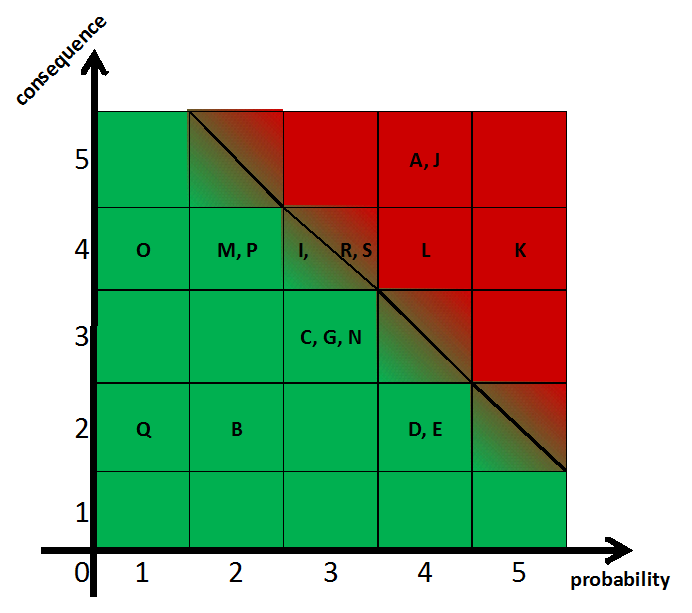
\includegraphics[scale=0.6]{./graphics/cxp}
\caption{Consequence \& probability diagram with placed risks}
\label{cxp}
\end{figure} % still missing
\todo[inline, color=red!50]{Risk analysis section is missing}
\subsection{Budget}
\label{budget_label}
The budget has been divided into a development budget and a operation budget. 
The development budget in table \ref{devbud} shows how much money we need for our concept to be ready for production. 
We assume that if we don't get any funding then the bank loan during the development phase will be with exempt from payments until we start production. 

The main costs of the development budget is the wages, establishing, rent and some unexpected costs. 
The basis: \begin{itemize}
\item[-] for the wage is that the team (7 persons) will be working full-time (160,33 h/month) to a wage equal to the minimum salary for a third year student (172 DDK/h\cite{ida-salary}).
\item[-] for establishing is covering office fittings (37000 DKK) and application for a patent/registration.
\item[-] for rent is a price check for renting commercial premises in Odense, Denmark. Premises with plenty of space is available at 5000 DKK.\cite{rent_prices}
\item[-] for the interest of the bank loan of 7 \% is that the concept is with some risks \ref{risk} , if there were no risks the interest would be lower. 
\end{itemize} 
The cost are listed in table \ref{devbud}, a full description can be found in appendix \ref{detailed_budget}. As it appears in the table we need 2,709,474 DKK to develop our concept. If no funding is granted a bank loan of 2.750.000 should be sufficient.

\begin{table}[h!]
\centering
\begin{tabular}{l r}
Development budget      & (DKK)              \\
\hline                                       
Variable costs:         &                    \\
Bill of materials       &    28,500        \\
Regular costs:          &                           \\
Wage                    &    2,316,448           \\
Rent                    &    75,000          \\
Establishment           &    87,000          \\
Others                  &    79,000          \\
Unexpected costs (5\%)  &    123,527         \\
\hline                      
Total                   &    2,709,474           \\
\end{tabular}
\caption{Summary of development budget}
\label{devbud}
\end{table}

The operation budget shows the cash-flow when we start producing and selling our product. We have made a budget for the first two years after the development phase. The operation budget consist of turnover, variable costs, regular costs and the bank loan if no funding is provided. We have made the following assumptions:
\begin{itemize}
\item[-] The first year we guess around 60 units and the next year around three times as much.
\item[-] Bill of materials is proportional with units sold.
\item[-] Regular cost stays the same as during the development phase.
\item[-] 7 percent in annual interest on bank loan because there is some risks. The payback is 40.000 per month. This gives a payback time on approximately 6 years.
\end{itemize}
A summery of the operation budget is shown in table \ref{opebud}, a full description can be found in appendix \todo[inline]{Budget: ref}.
\begin{table}[h!]
\centering
\begin{tabular}{l r r r r}
Operation budget      &            &              &             &    \\
                      & year 1     & year 2       & year 3      &    \\
\hline                                                               
Units sold            &          0 &        60   &         114  &    \\
Personnel             &          7 &         7   &          13  &    \\ 
\hline                                              
Turnover              &          0 & 4,800,000   &   9,120,000  & DKK\\
Variable costs        &     28,500 & 2,453,040   &   4,660,776  & DKK\\
Regular costs         &  2,685,324 & 1,798,032   &   3,180,666  & DKK\\
Bank loan (7\%)       &  3,056,026 & 3,047,532   &   2,297,787  & DKK\\
Payback               &          0 &   240,000   &     960,000  & DKK\\
Balance               &    136,092 &   213,429   &     321,576  & DKK\\  
% \hline                                                        
% Total                 &             &          &            \\
\end{tabular}
\caption{Summary of operation budget}
\label{opebud}
\end{table}


\begin{thebibliography}{9}
\bibitem{Control_Theory}
	Dorf and Bishop,
	Modern Control Systems,
	Prentice Hall, 
	12th edition, 
	2011.

	\bibitem{ida-salary}
	http://english.ida.dk/salary/minimum-salary,
	11 november,
	2014.
	
	\bibitem{rent_prices}
	http://www.lokalebasen.dk/leje/erhvervslokaler,
	17 november,
	2014.
	
	\bibitem{welding_salary}
	http://www.danskmetal.dk/Loen\%20og\%20arbejdsforhold/Loen/Loenstatistik.aspx \\
	Numbers based on the union ``Dansk Metal'' for ``Metal Odense'' in ``Smede og Stålkonstruktioner'',
	17 november,
	2014. 
	
	\bibitem{valk_welding_summary}
	Based on the meeting we had with Valk Welding.
	The summary can be found in appendix \ref{Valk_meeting_resume}
	
\end{thebibliography}

\part{Appendices}
\appendix
\addtocontents{toc}{\protect\setcounter{tocdepth}{1}}% Depth of appendix in table of content
\captionsetup{list=no}%remove figures from appendix on list of content
%%%%% Appendices should go here %%%%%%%
\section{Appendix: Pricing of Tool}
For the success of this product it is crucial that the price stays competitive. Offline programming methods currently in use today\footnote{Information courtesy of Valk Welding} costs 100.000Dkk for the software and required training. Our product should stay within this budget or offer significant advantages over competition.
\subsection{Bill of Materials}
In figure \ref{tab:BoM} is a rough estimate of the budget for each component needed to produce the robot. All of the prices are based on average costs of typical industrial range products in each category.  

\begin{figure}[h]
	\begin{center}
		\begin{tabular}{l c r}
		Product            & & Budget (DKK)\\
		\hline
		Camera 				& : & 5.000  \\
		Laser scanner		& : & 5.000 \\
		Custom Housing		& : & 5.000\\
		Embedded Hardware	& : & 2.000\\
		Software/Firmware	& : & 5.000\\
		UV flash			& : & 2.000\\
		Interface			& : & 3.000\\
		Marker				& : & 500\\[0.2cm]
		\hline
		Total				& : & 28.500\\ 
		\end{tabular}
	\end{center}
	\caption{Estimated bill of materials}
\label{tab:BoM}
\end{figure}
Some of the components mentioned in figure \ref{tab:BoM} require some elaboration:
\paragraph{Custom Housing:}
As previously mentioned most of the components used to manufacture this product already exist, making the manufacturing of the product mostly an assembly. However, a custom housing to hold the components as well as protect them from the potentially harsh conditions of a welding environment must be made. A design will be made inhouse and a machine shop [Real name?] will be hired to manufacture the housing.
\paragraph{Embedded Hardware:}
In order to provide the robot with the necessary information to perform a quality weld, it is necessary to include some hardware for managing the image processing as well as a range of other tasks. There are many off-the-shelf [off/of?] solutions on the market today, one of which is expected to meet the processing-needs of our application. If this is not the case or if it is economically advantagous, a custom processing board will be developed, in either case the assumed maximum budget is unaltered.
\paragraph{Software/Firmware:}
In order to realise this product a multitude of different programming tasks must be completed, naturally, the development costs must be included in the final price of the product.
\subsection{Manufacturing Cost}
Having bought all of the parts it is still necessary to assemble, test and paint each product. It will take an estimated 100 \todo[inline]{how many hours was it? 73?} manhours from parts to final product. Working at an engineers minimum wage this translates to 12.000Dkk.\todo[inline]{verify}
\subsection{Final Cost}
Taking into account both the BoM and the manufacturing cost, the total expenses of manufacturing the product reaches 40.500Dkk. \todo[inline]{Should we conclude on the final cost (80000) here? it seems malplaced..}
\clearpage
\section{Student-to-Student Teaching}
\subsection{Nikolaj}
I am studying robotic systems and as part of my education I had a course on classical control theory.

Control theory works with creating models and controllers for linear systems.
\subsubsection{Session topics}
The quick intro touched on what control diagrams looked like and how open loop and closed loop systems behave on an intuitive level.

To show an example of where transfer functions exist in the real world, the transfer function for a motor was calculated.
We talked about the different ways to represent a transfer function.
Stability was defined and examples of unstable systems was given.
We talked about how to read a pole zero transfer function and what pole positions meant for stability and how it affects the system in the time domain.
We talked about overshoot, damping and settling time.
We talked about what second order systems look like in the time domain.
Then an example was calculated to show how you would design a controller given requirements to it's performance in the time domain.

\begin{figure}[h]
\centering
\begin{subfigure}[c]{0.4\textwidth}
\centering
  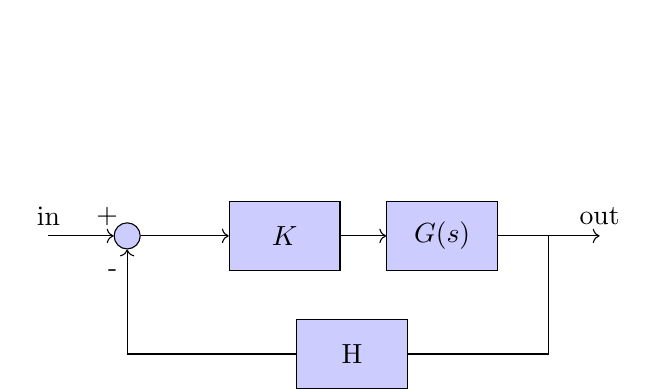
\begin{tikzpicture}[node distance = 2 cm]
  \node [input, name=input] {};
\node [sum,right of= input](sum) {};
\node [block, right of=sum] (K) {\(K\)};
\node [block, right of=K] (sys) {\(G(s)\)};
\node [output, right of= sys] (output){};

\draw[->] (input) -- node[pos=0.9, above] {+} (sum);
\draw[->] (sum) -- (K);
\draw[->] (K) -- (sys);
\draw[->] (sys) -- node[name=feedback] {} (output);

\node at (0,2) {} ;
\node at (0,-2) {} ;

\node[yshift=0.25cm] at (input) {in};
\node[yshift=0.25cm] at (output) {out};
\draw[->] (feedback.center) |- ++(-2.5,-1.5) node[block, name=H] {H};
\draw[->] (H) -| node[pos=0.9, left] {-} (sum);
  \end{tikzpicture}
  \caption{closed loop system}
\end{subfigure}
\begin{subfigure}[c]{0.4\textwidth}
\centering
  \begin{tikzpicture}
    \draw
      (0,-1) -- (0,1) node[above] {\(j\omega\)}
      (-4,0) -- (1,0) node[right] {\(\sigma\)}
    ;

    \node[pole] at (-1,0) {};
    \node[pole] at (-2,0) {} ;
    \node[pole] at (-3,0) {} ;
    
    \draw[dashed,->] (-2,0) -- (0,3.46);
    \draw[dashed,->] (-2,0) -- (0,-3.46);
    \draw (-1.5,0) arc(0:60:0.5);
    
    \draw[very thick] (-2,0) -- (-1.5,0) to[out=90, in=240] (-1,1.73) -- (0,3.46);
    \draw[very thick] (-1,0) -- (-1.5,0) to[out=-90, in=-240] (-1,-1.73) -- (0,-3.46);
    \draw[very thick,->] (-3,0) -- (-3.9,0);
  \end{tikzpicture}
  \caption{Root Locus}
\end{subfigure}
\caption{Topics introduced in ``student to student'' teaching about control theory}
\end{figure}

Root Locus was defined and it was shown how to read a Root Locus plot and how to draw it by hand. 
We talked about PID controllers and what the parameters meant. 
We talked about systems that uses PID in the real world.
We talked about ways to chose parameters for PID using the Zigler Nichols method.

\subsubsection{Evaluation}
A lot of topics were chosen and it was impossible to get explore a single topic withe the given time constraints.

This made it possible to give an overview so people with little to no prior knowledge of control theory could visualize what is possible and how to design a controller.

The used math was not explained in this session as all the students knew about this already.

This was well received and people seemed to follow the conclusions without going into detail about Laplas transforms and second order systems.

The illustrations used was either examples from the book \todo[inline]{name and number} or drawn myself.

There were a lot of questions during the presentation which shows that they were interested in the subject

The response to the session was that it was a bit more technical than they expected. 
But the pace was fine and it was easy to follow. 





a. Topics of your session. 
b. Evaluation of the session in general, the teaching materials, the relevance of the topics and planning and conduction of the session. 
c. The material used in the session might be enclosed in Appendix. 

Documentation and feedback on/evaluation of your lessons from your team
members must be included in the project report by each subgroup of
students.  %first appendix should be input, rest should be include
\newpage
\subsection{Thomas Søndergaard Christensen}
As a part of Experts in Teams we were required to teach a topic relevant to the development process of our product to the team. My main field being robotics, I decided to teach the topic of robot motion planning. My goal was to give an overview of the basic techniques used to plan robot motion, as well as some of the difficulties that you may be faced with when planning robot motion.
\subsubsection{Session Topics}
Initially a (very) brief overview of the different types of robots was given, three examples were used: Robot arms from the automotive industry, simple robot vacuum cleaners and finally, a team of football-playing robots competing for the Robocup.
Two very commonly used terms in robotics are the work-space and configuration-space of a robot. Using the example of a robot capable of motion in 2D space I explained the usefulness and limitations of the two concepts. Additionally I explained (or attempted to) the implications to the configuration-space of adding an obstacle in the work-space of a robot.
Lastly I presented the wavefront algorithm, explaining its workings and showing examples of applications used in class.
\subsubsection{Evaluation}
\paragraph{Group:}~\\
Generally people found the structure of the teaching session logical and easily understood. Additionally, the examples given were well-received and made a good job of describing the concepts. Some hinted that the difficulty could have been increased without it being an issue.
\paragraph{Own Reflections:}~\\
When deciding what material to include and what not to include I found it difficult to determine what level i would be teaching at. Given the limited time of the presentation, I did not want to attempt teaching subjects that require that some knowledge about robotic motion is already present. While my team did not necessarily have knowledge about my chosen subject in advance, they had had courses dealing with similar issues prior to my teaching session.\\
My experience from earlier student-to-student teachings told me that there would be many questions during the session, this led me to choose to  limit the length of my presentation to roughly 30 minutes, allowing time for questions. However, not a single question was asked during the presentation, meaning that my session fell short of the allowed 45 minutes. In hindsight I should have included an extra topic in case of the event that no questions were asked.\\
In general I am satisfied with the outcome of my teaching session. I believe the information was relevant to the project at hand and it was well received by my team.

% \include{./content/Appendix/}
\end{document} 